% ═══════════════════════════════════════════════════════════════
%  Weekly Meeting - 17 April 2026
%  Beam-Path Heterogeneity Metrics & Energy-Stratified Correlation
%  Author: Mikołaj Stryja
% ═══════════════════════════════════════════════════════════════
\documentclass[aspectratio=169, 10pt]{beamer}

% ── Theme & colours ─────────────────────────────────────────
\usetheme{Madrid}
\usecolortheme{default}
\definecolor{tudelft}{RGB}{0,100,172}
\setbeamercolor{structure}{fg=tudelft}
\setbeamercolor{title}{fg=white,bg=tudelft}
\setbeamercolor{frametitle}{fg=white,bg=tudelft}
\setbeamertemplate{navigation symbols}{}
\setbeamertemplate{footline}{%
  \leavevmode\hbox{%
    \begin{beamercolorbox}[wd=.33\paperwidth,ht=2.5ex,dp=1ex,center]{author in head/foot}%
      \usebeamerfont{author in head/foot}\insertshortauthor
    \end{beamercolorbox}%
    \begin{beamercolorbox}[wd=.34\paperwidth,ht=2.5ex,dp=1ex,center]{title in head/foot}%
      \usebeamerfont{title in head/foot}\insertshorttitle
    \end{beamercolorbox}%
    \begin{beamercolorbox}[wd=.33\paperwidth,ht=2.5ex,dp=1ex,right]{date in head/foot}%
      \usebeamerfont{date in head/foot}\insertframenumber{}/\inserttotalframenumber\hspace*{2ex}
    \end{beamercolorbox}}%
  \vskip0pt%
}

% ── Packages ────────────────────────────────────────────────
\usepackage{graphicx}
\usepackage{booktabs}
\usepackage{amsmath,amssymb}
\usepackage{siunitx}
\usepackage{tikz}
\usetikzlibrary{arrows.meta,positioning,calc,shadows.blur}
\usepackage{xcolor}
\usepackage{multirow}
\usepackage{algorithm2e}
\graphicspath{{figures/}}

% ── Meta ────────────────────────────────────────────────────
\title[ADoTA Heterogeneity Analysis]{Beam-Path Heterogeneity Metrics\\[4pt]
{\small Correlation with GPR \& Energy-Stratified Analysis ($n = 3\,950$)}}
\author[M.~Stryja]{Mikołaj Stryja}
\institute{Department of Radiation Science \& Technology}
\date{17 April 2026}

% ════════════════════════════════════════════════════════════
\begin{document}

% ── Title ───────────────────────────────────────────────────
\begin{frame}[plain]
  \titlepage
\end{frame}

% ── Outline ─────────────────────────────────────────────────
\begin{frame}{Outline}
  \tableofcontents
\end{frame}

% ════════════════════════════════════════════════════════════
\section{Recap \& New Approach}
% ════════════════════════════════════════════════════════════

\begin{frame}{Recap \& New Approach}
  \textbf{Last week}: spherical neighbourhood around BP $\rightarrow$
  $\sigma_{\text{HU}}$, TV, CV as heterogeneity metrics.

  \vspace{6pt}
  \textbf{Limitation}: a single sphere ignores \emph{where} along the beam
  path the density transitions occur.

  \vspace{6pt}
  \textbf{This week: extended pipeline}
  \begin{enumerate}
    \item \textbf{Density region analysis}: segment beam path into contiguous
          tissue regions inside the BP range.
    \item \textbf{Six advanced heterogeneity metrics}: max HU jump,
          $\sigma_{\text{HU}}$ at BP, max HU gradient, lateral HU variance,
          heterogeneity fraction, interface--BP distance.
    \item \textbf{Two 3-D Sobel edge metrics}: mean axial Sobel magnitude
          and 95th-percentile Sobel in the BP region.
    \item \textbf{Energy-stratified correlation analysis}: binned
          correlations, energy-coloured scatter plots, and partial
          correlations controlling for beam energy.
  \end{enumerate}

  \vspace{4pt}
  {\small Dataset: $n = 3\,950$ beamlets from the ADoTA training set,
  beam energies \SIrange{70}{250}{MeV}.}
\end{frame}

% ════════════════════════════════════════════════════════════
\section{CT Segmentation}
% ════════════════════════════════════════════════════════════

\begin{frame}{Tissue Segmentation: HU Look-Up Table}
  Each CT voxel is assigned to one of \textbf{7 tissue classes} based on its
  Hounsfield Unit value.

  \vspace{6pt}
  \begin{center}
    \begin{tabular}{clcc}
      \toprule
      \textbf{Class} & \textbf{Label} & \textbf{HU range} & \textbf{Colour} \\
      \midrule
      0 & Air            & $[-1024,\; -950)$ & black \\
      1 & Lung           & $[-950,\; -500)$  & dark blue \\
      2 & Fat            & $[-500,\; -100)$  & cyan \\
      3 & Soft tissue    & $[-100,\; 100)$   & green \\
      4 & Contrast/blood & $[100,\; 300)$    & yellow \\
      5 & Cancellous bone& $[300,\; 500)$    & orange \\
      6 & Cortical bone  & $[500,\; 3072)$   & red \\
      \bottomrule
    \end{tabular}
  \end{center}

  \vspace{6pt}
  Implementation: \texttt{segment\_hu()} iterates over the LUT and assigns
  the class index whose HU interval contains the voxel value.

  \vspace{4pt}
  {\small Boundaries derived from the Hounsfield scale reference values
  (\url{https://en.wikipedia.org/wiki/Hounsfield_scale}) and verified
  against clinical tissue classification ranges.}
\end{frame}

% ════════════════════════════════════════════════════════════
\section{Gaussian Smoothing}
% ════════════════════════════════════════════════════════════

\begin{frame}{Gaussian Smoothing of CT Before Segmentation}
  \textbf{Problem}: raw CT volumes contain acquisition noise. Direct
  segmentation on raw data can produce noisy class maps with many
  spurious small connected regions, inflating the density region count.

  \vspace{8pt}
  \textbf{Solution}: apply a 3-D Gaussian filter before segmentation.
  Conceptually,
  \begin{equation*}
    \tilde{I}(\mathbf{r}) \;=\; \bigl(G_\sigma * I\bigr)(\mathbf{r}),
    \qquad
    G_\sigma(\mathbf{r}) \;=\;
    \frac{1}{(2\pi\sigma^2)^{3/2}}
    \exp\!\Bigl(-\frac{|\mathbf{r}|^2}{2\sigma^2}\Bigr)
  \end{equation*}
  On the voxel grid, this is implemented numerically as a discrete
  separable convolution along each axis.

  \vspace{4pt}
  \begin{itemize}
    \item Implementation:
    \texttt{from scipy.ndimage import gaussian\_filter}
    \\
    \texttt{ct\_hu\_smooth = gaussian\_filter(ct\_hu, sigma=1.0, mode='reflect')}
    \item \(\sigma = 1.0\) voxel \(= \SI{2}{mm}\) for a
    \(2 \times 2 \times \SI{2}{mm}\) grid.
    \item Effect: suppresses high-frequency noise and reduces spurious
    small regions before segmentation.
    \item Result: density region count better reflects anatomical
    structure rather than voxel-scale noise.
  \end{itemize}
\end{frame}

% ════════════════════════════════════════════════════════════
\section{Bragg Peak Range Estimation}
% ════════════════════════════════════════════════════════════

\begin{frame}{Bragg Peak Range from Ground-Truth IDD}
  \textbf{Integrated Depth Dose (IDD)}: collapse the 3-D dose to 1-D:
  \begin{equation*}
    \text{IDD}[k] \;=\; \sum_{y}\sum_{x} D[k, y, x], \qquad k = 0, \ldots, N_z - 1
  \end{equation*}

  \textbf{Bragg peak index}: $k^* = \arg\max_k \;\text{IDD}[k]$

  \vspace{6pt}
  \textbf{Proximal boundary} $z_{\min}$: walk \emph{backward} from $k^*$
  towards the entrance:
  \begin{equation*}
    z_{\min} = \max\bigl\{\, k \leq k^* \;\big|\;
    \text{IDD}[k] < 0.50 \cdot \text{IDD}_{\max} \,\bigr\}
  \end{equation*}
  {\small Anchored to the peak, robust against entrance plateau noise.
  Analogous to clinical proximal R50.}

  \vspace{6pt}
  \textbf{Distal boundary} $z_{\max}$: walk \emph{forward} from $k^*$:
  \begin{equation*}
    z_{\max} = \min\bigl\{\, k \geq k^* \;\big|\;
    \text{IDD}[k] < 0.10 \cdot \text{IDD}_{\max} \,\bigr\}
  \end{equation*}
  {\small Marks the distal fall-off at 10\% of peak dose.}

  \vspace{4pt}
  Physical units: $z_{\min/\max}[\text{mm}] = z_{\min/\max}[\text{slices}]
  \times \SI{2}{mm/slice}$.
\end{frame}

% ════════════════════════════════════════════════════════════
\section{Density Region Analysis}
% ════════════════════════════════════════════════════════════

\begin{frame}{Density Region Analysis: Overview}
  \textbf{Goal}: characterise \emph{how many tissue transitions} the beam
  traverses inside the Bragg peak zone.

  \vspace{6pt}
  \begin{columns}[T]
    \begin{column}{0.55\textwidth}
      \textbf{Steps:}
      \begin{enumerate}
        \item For each depth slice $k \in [z_{\min}, z_{\max}]$, compute the
              \textbf{flux-weighted mean HU}:
              \begin{equation*}
                \bar{H}[k] = \frac{\sum_{y,x} w_{k,y,x}\, I_{k,y,x}}
                                   {\sum_{y,x} w_{k,y,x}}
              \end{equation*}
              where $w_{k,y,x} = |\text{flux}[k,y,x]|$ if
              $\geq 0.10 \cdot \max_{\!y,x}|\text{flux}[k]|$, else $0$.
        \item Segment $\bar{H}[k]$ into tissue class $c[k]$ using the HU LUT.
        \item Group consecutive slices with the \textbf{same class} into
              contiguous \textbf{density regions}.
      \end{enumerate}
    \end{column}
    \begin{column}{0.42\textwidth}
      \begin{center}
        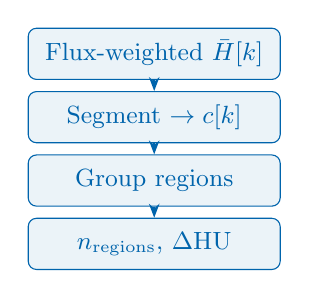
\begin{tikzpicture}[
          box/.style={draw=tudelft, rounded corners=3pt,
                      minimum width=3.2cm, minimum height=0.65cm,
                      font=\small, text=tudelft, fill=tudelft!8},
          arr/.style={-{Stealth[length=5pt]}, thick, tudelft}
        ]
          \node[box] (whu) {Flux-weighted $\bar{H}[k]$};
          \node[box, below=4pt of whu] (seg) {Segment $\rightarrow c[k]$};
          \node[box, below=4pt of seg] (grp) {Group regions};
          \node[box, below=4pt of grp] (met) {$n_{\text{regions}}$, $\Delta$HU};
          \draw[arr] (whu) -- (seg);
          \draw[arr] (seg) -- (grp);
          \draw[arr] (grp) -- (met);
        \end{tikzpicture}
      \end{center}
    \end{column}
  \end{columns}
\end{frame}

\begin{frame}{Density Region Analysis: Metrics}
  \textbf{Two output metrics per beamlet:}

  \vspace{8pt}
  \textbf{1.\ Number of density regions} ($n_{\text{regions}}$):\\[2pt]
  Count of maximal contiguous groups of slices sharing the same tissue class
  along the beam path inside $[z_{\min}, z_{\max}]$.

  \vspace{4pt}
  {\small Example: Soft tissue $\rightarrow$ Bone $\rightarrow$ Soft tissue
  $= 3$ regions.}

  \vspace{10pt}
  \textbf{2.\ Total HU change} ($\Delta_{\text{total}}$):\\[2pt]
  Sum of absolute mean-HU differences between consecutive regions:
  \begin{equation*}
    \Delta_{\text{total}} = \sum_{j=1}^{n_{\text{regions}}-1}
    \bigl|\, \bar{H}_j - \bar{H}_{j-1} \,\bigr|
  \end{equation*}
  where $\bar{H}_j$ is the mean HU of region~$j$.

  \vspace{8pt}
  \textbf{Hypothesis}: higher $n_{\text{regions}}$ and/or
  $\Delta_{\text{total}}$ $\longrightarrow$ harder sample
  $\longrightarrow$ lower GPR.
\end{frame}

\begin{frame}[fragile]{Density Region Analysis: Pseudocode}
  \vspace{-2pt}
  \begin{center}
  \scalebox{0.85}{%
  \begin{minipage}{0.95\textwidth}
  \begin{algorithm}[H]
    \DontPrintSemicolon
    \SetAlgoLined
    \KwIn{CT volume $I \in \mathbb{R}^{D \times H \times W}$,
          flux $F \in \mathbb{R}^{D \times H \times W}$,
          BP range $[z_{\min}, z_{\max}]$}
    \KwOut{$n_{\text{regions}}$, $\Delta_{\text{total}}$}
    \BlankLine
    \For{$k \leftarrow \lceil z_{\min} \rceil$ \KwTo $\lfloor z_{\max} \rfloor$}{
      $f_{\max} \leftarrow \max_{y,x} |F[k,y,x]|$ \;
      $\text{mask} \leftarrow |F[k]| \geq 0.10 \cdot f_{\max}$ \;
      $\bar{H}[k] \leftarrow \text{weighted\_avg}\bigl(I[k,\text{mask}],\;
        |F[k,\text{mask}]|\bigr)$ \;
    }
    $c[k] \leftarrow \textsc{SegmentHU}\bigl(\bar{H}[k]\bigr)$
      \tcp*{tissue class per slice}
    Group consecutive slices with same $c[k]$ into regions
      $R_0, R_1, \ldots$ \;
    $n_{\text{regions}} \leftarrow$ number of regions \;
    $\Delta_{\text{total}} \leftarrow
      \sum_{j=1}^{n_{\text{regions}}-1} |\bar{H}_j - \bar{H}_{j-1}|$ \;
    \Return{$n_{\text{regions}},\; \Delta_{\text{total}}$}
  \end{algorithm}
  \end{minipage}
  }
  \end{center}
\end{frame}

% ════════════════════════════════════════════════════════════
\section{Example: CT Segmentation \& IDD}
% ════════════════════════════════════════════════════════════

{
\setbeamertemplate{footline}{}
\begin{frame}[plain]{Example Beamlet: CT Segmentation, Sobel Edges \& IDD}
  \vspace{-6pt}
  \begin{center}
    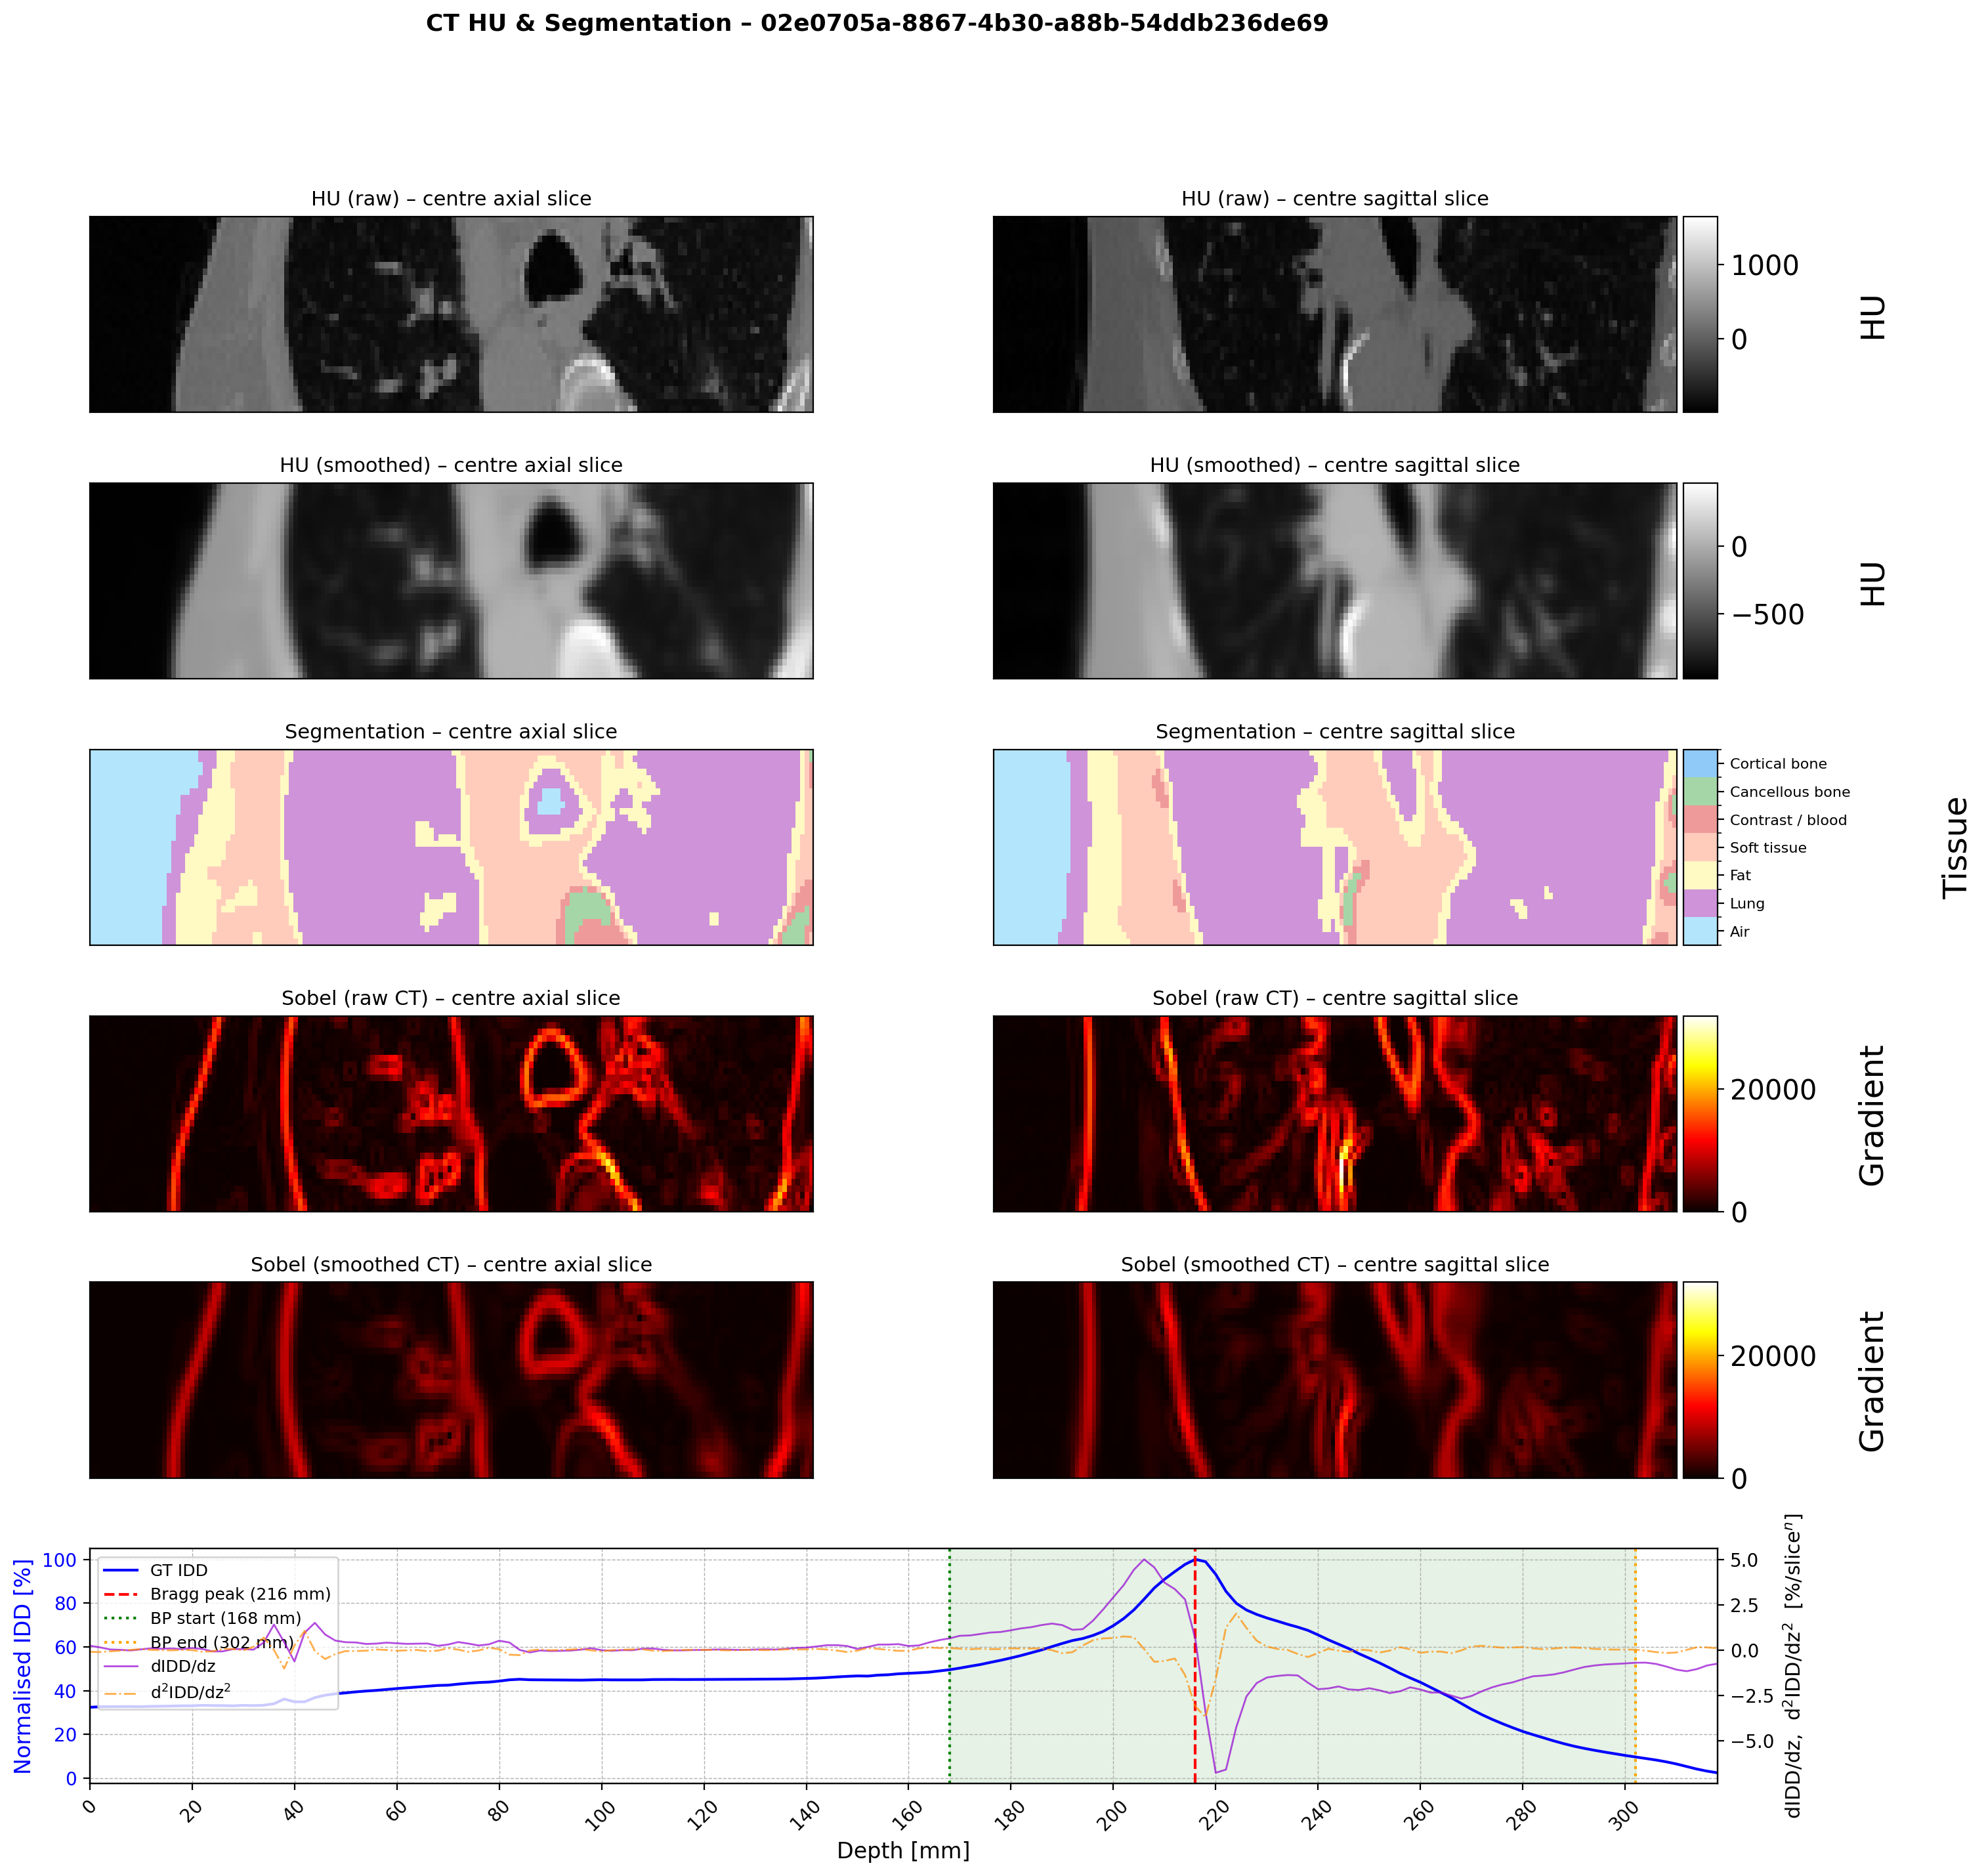
\includegraphics[width=\textwidth,height=0.82\textheight,keepaspectratio]{02e0705a-8867-4b30-a88b-54ddb236de69_ct_seg.png}
  \end{center}
  \vspace{-6pt}
  {\footnotesize Beamlet \texttt{02e0705a}, \SI{127.55}{MeV}.
  Row~1: raw CT.  Row~2: Gaussian-smoothed CT ($\sigma{=}1$ vox).
  Row~3: 7-class segmentation.  Row~4: raw Sobel magnitude.
  Row~5: smoothed Sobel magnitude.  Bottom: IDD with BP range
  (green: R50--R10).}
\end{frame}
}

% ════════════════════════════════════════════════════════════
\section{Example: ADoTA Dose Prediction}
% ════════════════════════════════════════════════════════════

{
\setbeamertemplate{footline}{}
\begin{frame}[plain]{Example Beamlet: ADoTA Dose Prediction}
  \vspace{-6pt}
  \begin{center}
    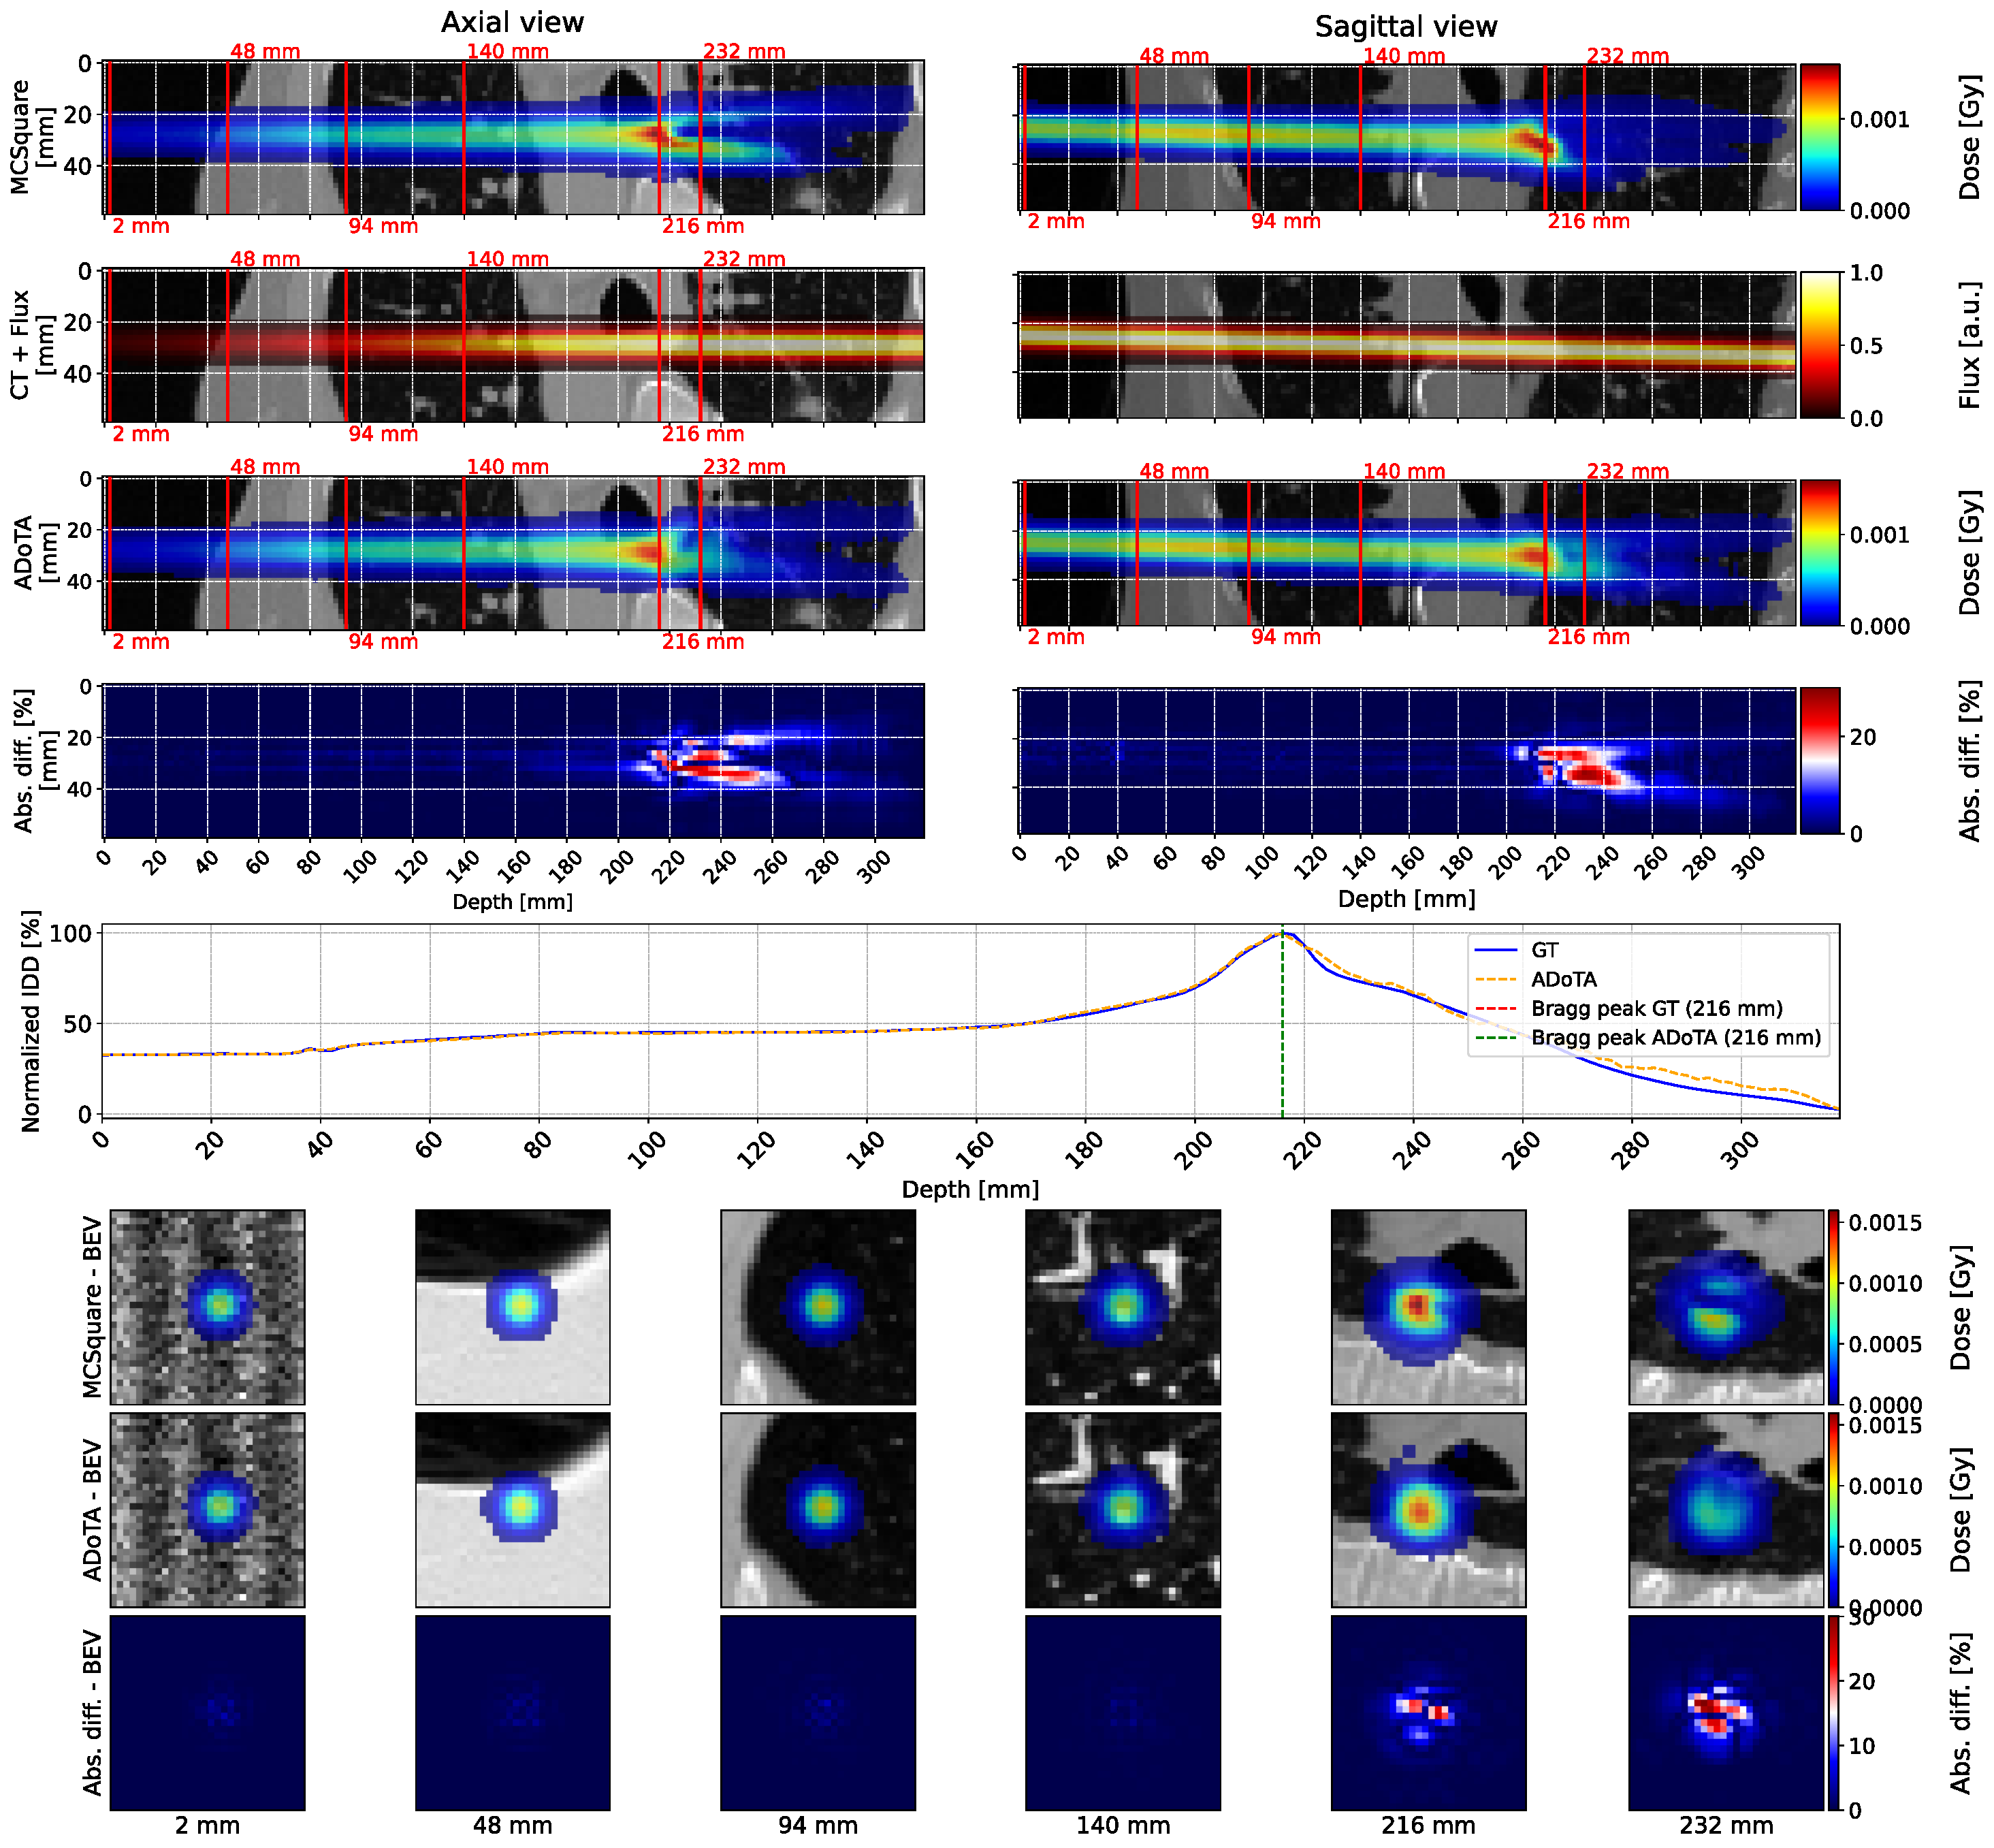
\includegraphics[width=\textwidth,height=0.82\textheight,keepaspectratio]{example_publication.pdf}
  \end{center}
  \vspace{-6pt}
  {\footnotesize Same beamlet.  Top: CT input \& beamlet shape (flux).
  Bottom: ground-truth dose (MC), ADoTA prediction, and gamma index
  map ($2\%/\SI{2}{mm}$).  Depth slices sampled uniformly from
  entrance to distal fall-off.}
\end{frame}
}

% ════════════════════════════════════════════════════════════
\section{Advanced Heterogeneity \& Sobel Metrics}
% ════════════════════════════════════════════════════════════

\begin{frame}{Advanced Heterogeneity Metrics}
  Six additional metrics computed along the beam path in the BP range:

  \vspace{4pt}
  \begin{center}
  \scalebox{0.88}{%
    \begin{tabular}{lll}
      \toprule
      \textbf{Metric} & \textbf{Symbol} & \textbf{Definition} \\
      \midrule
      Max HU jump & $\Delta H_{\max}$ & Largest $|\bar{H}_j - \bar{H}_{j-1}|$ between consecutive regions \\
      $\sigma_{\text{HU}}$ at BP & $\sigma_{\text{BP}}$ & Std.\ dev.\ of flux-weighted mean HU along BP slices \\
      Max HU gradient & $g_{\max}$ & $\max_k |\bar{H}[k+1] - \bar{H}[k]|$ (slice-to-slice) \\
      Lateral HU variance & $\text{Var}_{\perp}$ & Mean intra-slice HU variance within flux mask \\
      Heterogeneity fraction & $f_{\text{het}}$ & Fraction of BP slices with tissue class $\neq$ dominant class \\
      Interface--BP distance & $d_{\text{int}}$ & Distance (mm) from nearest tissue interface to $k^*$ \\
      \bottomrule
    \end{tabular}
  }
  \end{center}

  \vspace{6pt}
  \textbf{Rationale}: these metrics capture complementary aspects of tissue
  complexity: magnitude of transitions ($\Delta H_{\max}$, $g_{\max}$),
  overall variability ($\sigma_{\text{BP}}$, $\text{Var}_{\perp}$),
  spatial extent of heterogeneity ($f_{\text{het}}$), and proximity of
  interfaces to the dose-sensitive BP region ($d_{\text{int}}$).
\end{frame}

\begin{frame}{3-D Sobel Edge Detection Metrics}
  \textbf{Motivation}: Sobel operators detect tissue boundaries directly
  from the CT gradient, without requiring segmentation.

  \vspace{6pt}
  \textbf{Method}:
  \begin{enumerate}
    \item Smooth CT with Gaussian ($\sigma = 1.0$ voxel) to suppress noise.
    \item Apply 3-D Sobel filters along depth ($z$), height ($y$), and
          width ($x$) axes:
          \begin{equation*}
            S(\mathbf{r}) = \sqrt{S_z^2 + S_y^2 + S_x^2}
          \end{equation*}
    \item Aggregate within the flux-weighted beam path.
  \end{enumerate}

  \vspace{6pt}
  \textbf{Two output metrics:}
  \begin{itemize}
    \item \textbf{Mean axial Sobel} ($\bar{S}_{\text{axial}}$): flux-weighted
          mean of $|S_z|$ across the full beam path, capturing axial
          density transitions along the beam direction.
    \item \textbf{P95 Sobel at BP} ($S_{95,\text{BP}}$): 95th percentile of
          $S(\mathbf{r})$ within the BP range, weighted by flux,
          capturing the most extreme edge responses near the Bragg peak.
  \end{itemize}
\end{frame}

% ════════════════════════════════════════════════════════════
\section{Results: Overall Correlation with GPR}
% ════════════════════════════════════════════════════════════

\begin{frame}{Dataset \& Model Inference}
  \begin{columns}[T]
    \begin{column}{0.48\textwidth}
      \textbf{Dataset:}
      \begin{itemize}
        \item $n = 3\,950$ beamlets from the ADoTA training set
        \item Energy range: \SIrange{70}{250}{MeV}
        \item Grid: $160 \times 30 \times 30$ voxels,
              $2 \times 2 \times \SI{2}{mm}$
      \end{itemize}

      \vspace{6pt}
      \textbf{Model}: ADoTA v3 (DoTA\_v3\_grid\_search\_v11)\\
      Gamma pass rate: $2\%/\SI{2}{mm}$, 10\% lower dose cutoff

      \vspace{6pt}
      \textbf{GPR distribution:}\\
      Mean $= 98.81\%$, $\sigma = 1.49\%$\\
      Range: $[86.97\%,\; 100.00\%]$
    \end{column}
    \begin{column}{0.48\textwidth}
      \textbf{Energy bin distribution:}
      \vspace{4pt}
      \begin{center}
        \begin{tabular}{crc}
          \toprule
          \textbf{Bin (MeV)} & \textbf{$n$} & \textbf{GPR (\%)} \\
          \midrule
          70--100  & 892  & $98.33 \pm 2.02$ \\
          100--130 & 888  & $98.77 \pm 1.50$ \\
          130--160 & 1018 & $98.90 \pm 1.45$ \\
          160--190 & 781  & $99.27 \pm 0.77$ \\
          190--220 & 195  & $99.14 \pm 0.58$ \\
          220--250 & 176  & $98.59 \pm 0.80$ \\
          \bottomrule
        \end{tabular}
      \end{center}
      {\small Lower energies show larger GPR variance.}
    \end{column}
  \end{columns}
\end{frame}

\begin{frame}{Overall Correlation Ranking ($n = 3\,950$)}
  \begin{columns}[T]
    \begin{column}{0.42\textwidth}
      \vspace{-4pt}
      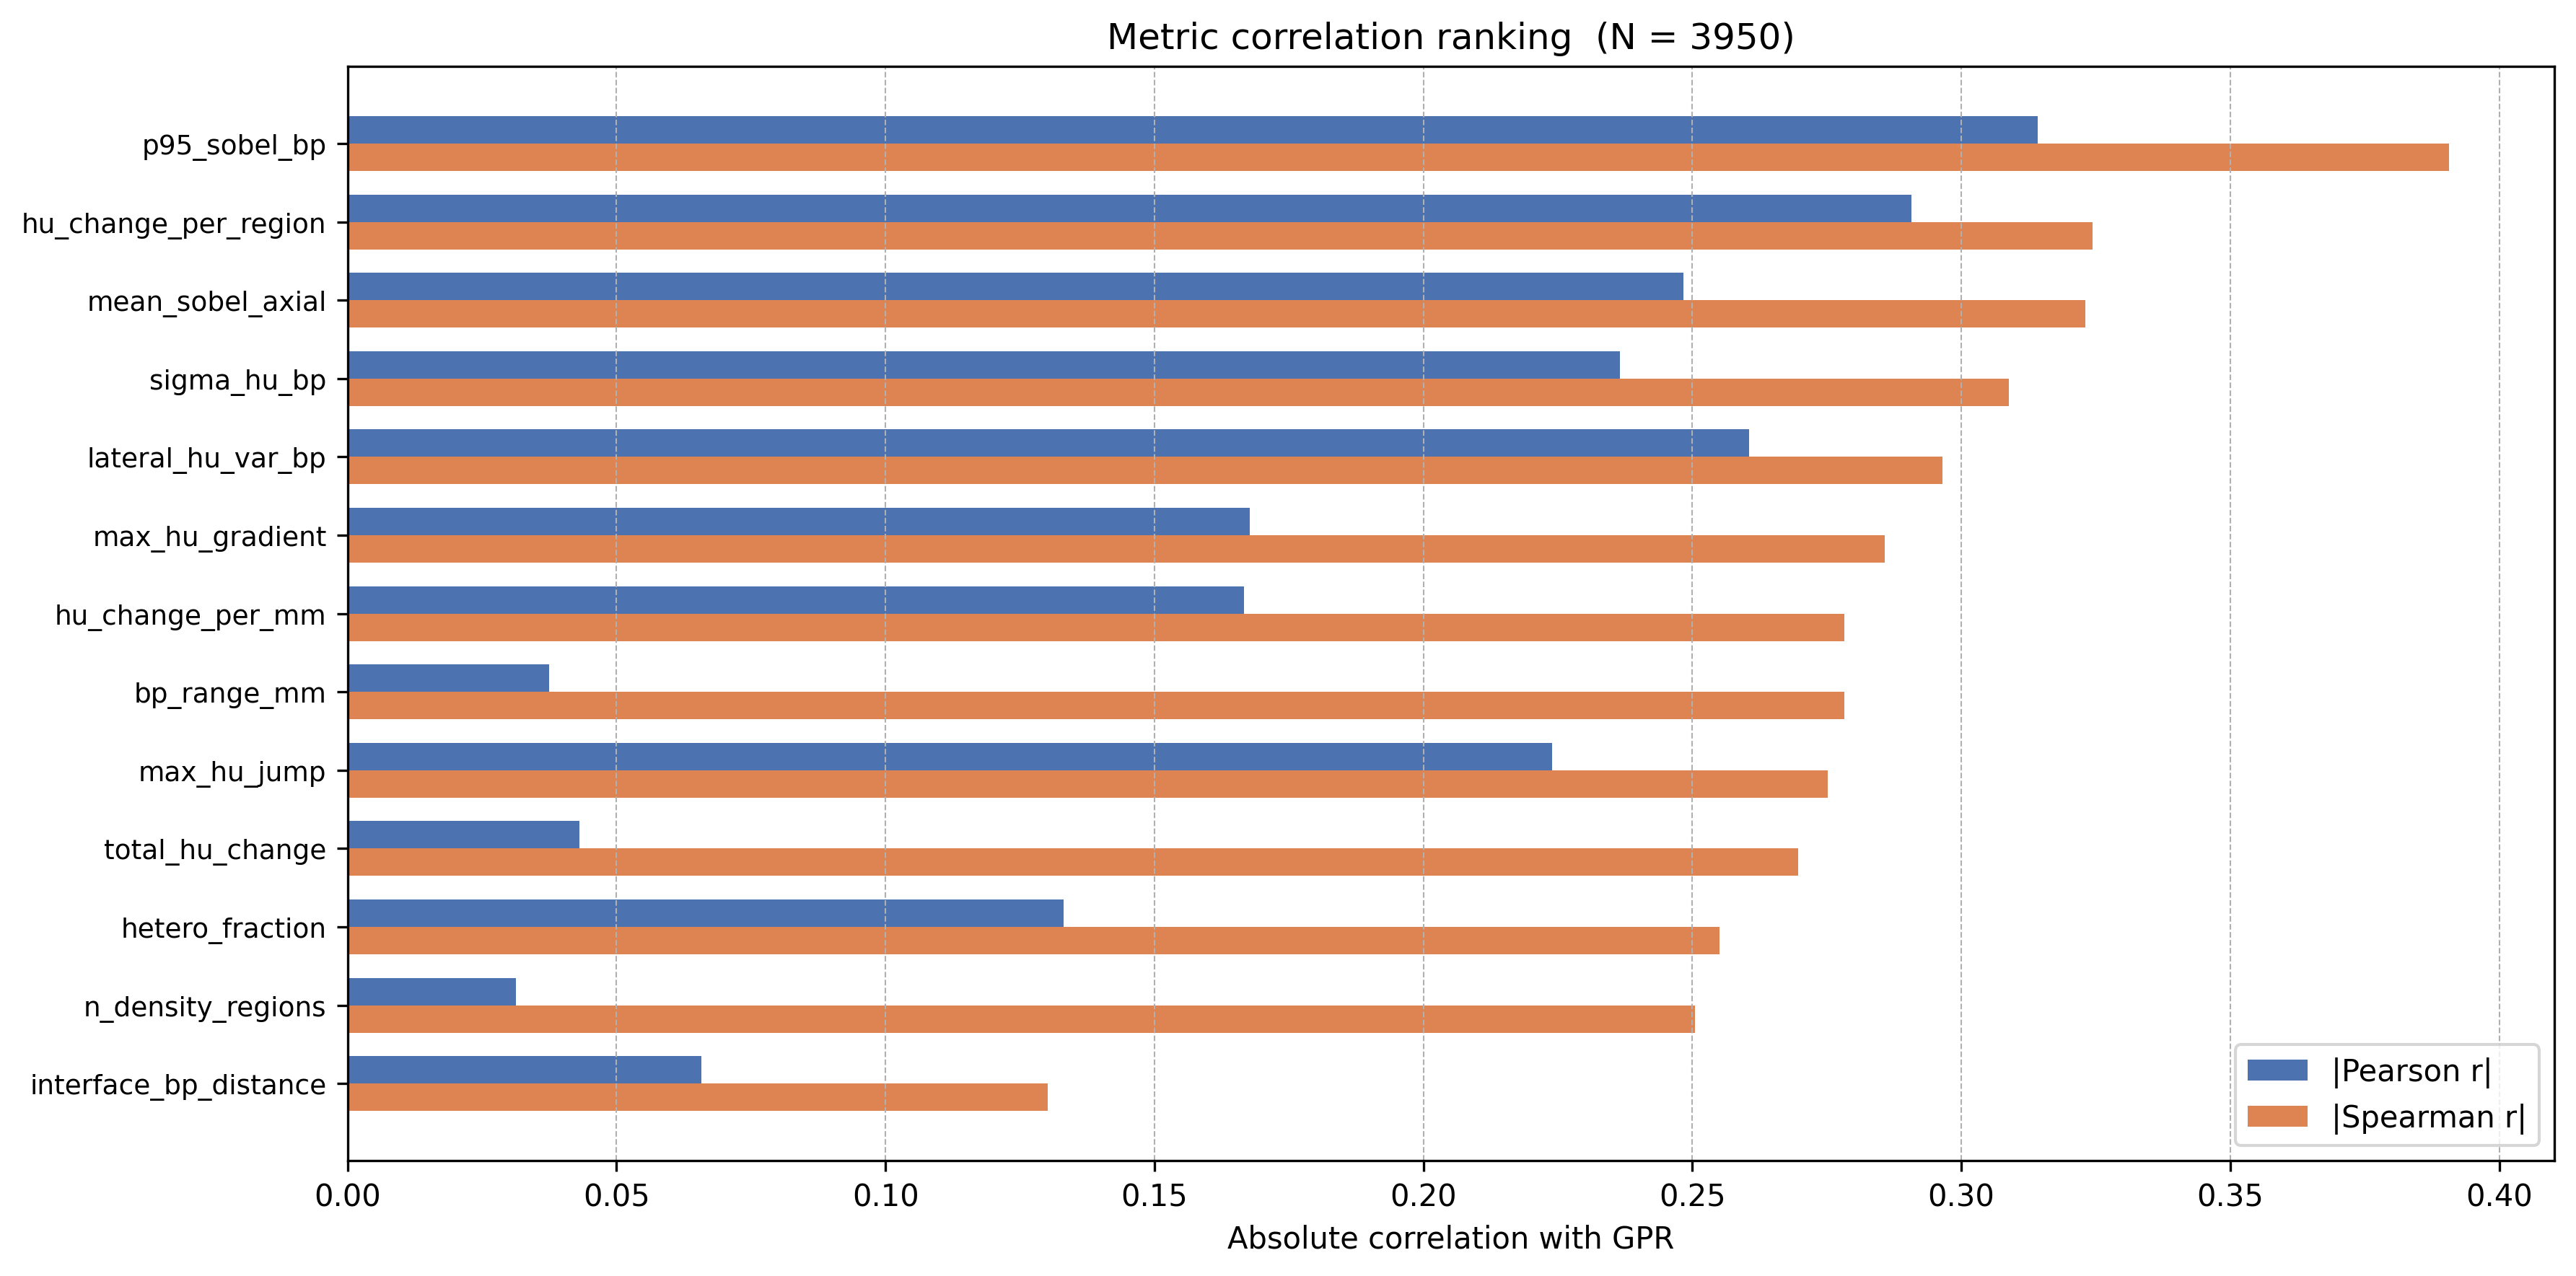
\includegraphics[width=\textwidth]{correlation_ranking.png}
    \end{column}
    \begin{column}{0.56\textwidth}
      \vspace{-2pt}
      {\small
      \begin{tabular}{lrr}
        \toprule
        \textbf{Metric} & \textbf{Spearman} & \textbf{Pearson} \\
        \midrule
        p95\_sobel\_bp          & $-0.391$ & $-0.314$ \\
        hu\_change\_per\_region & $-0.324$ & $-0.291$ \\
        mean\_sobel\_axial      & $-0.323$ & $-0.248$ \\
        $\sigma_{\text{HU}}$ at BP & $-0.309$ & $-0.237$ \\
        lateral\_hu\_var\_bp    & $-0.297$ & $-0.261$ \\
        max\_hu\_gradient       & $-0.286$ & $-0.168$ \\
        hu\_change\_per\_mm     & $-0.278$ & $-0.167$ \\
        bp\_range\_mm           & $-0.278$ & $-0.037$ \\
        max\_hu\_jump           & $-0.275$ & $-0.224$ \\
        total\_hu\_change       & $-0.270$ & $-0.043$ \\
        hetero\_fraction        & $-0.255$ & $-0.133$ \\
        $n_{\text{regions}}$    & $-0.251$ & $-0.031$ \\
        interface\_bp\_dist.    & $+0.130$ & $+0.066$ \\
        \bottomrule
      \end{tabular}
      }
      \vspace{4pt}

      {\small All $p < 10^{-5}$. Spearman $>$ Pearson suggests
      \textbf{monotonic but non-linear} relationships.}
    \end{column}
  \end{columns}
\end{frame}

\begin{frame}{Best Predictor: P95 Sobel at BP}
  \begin{center}
    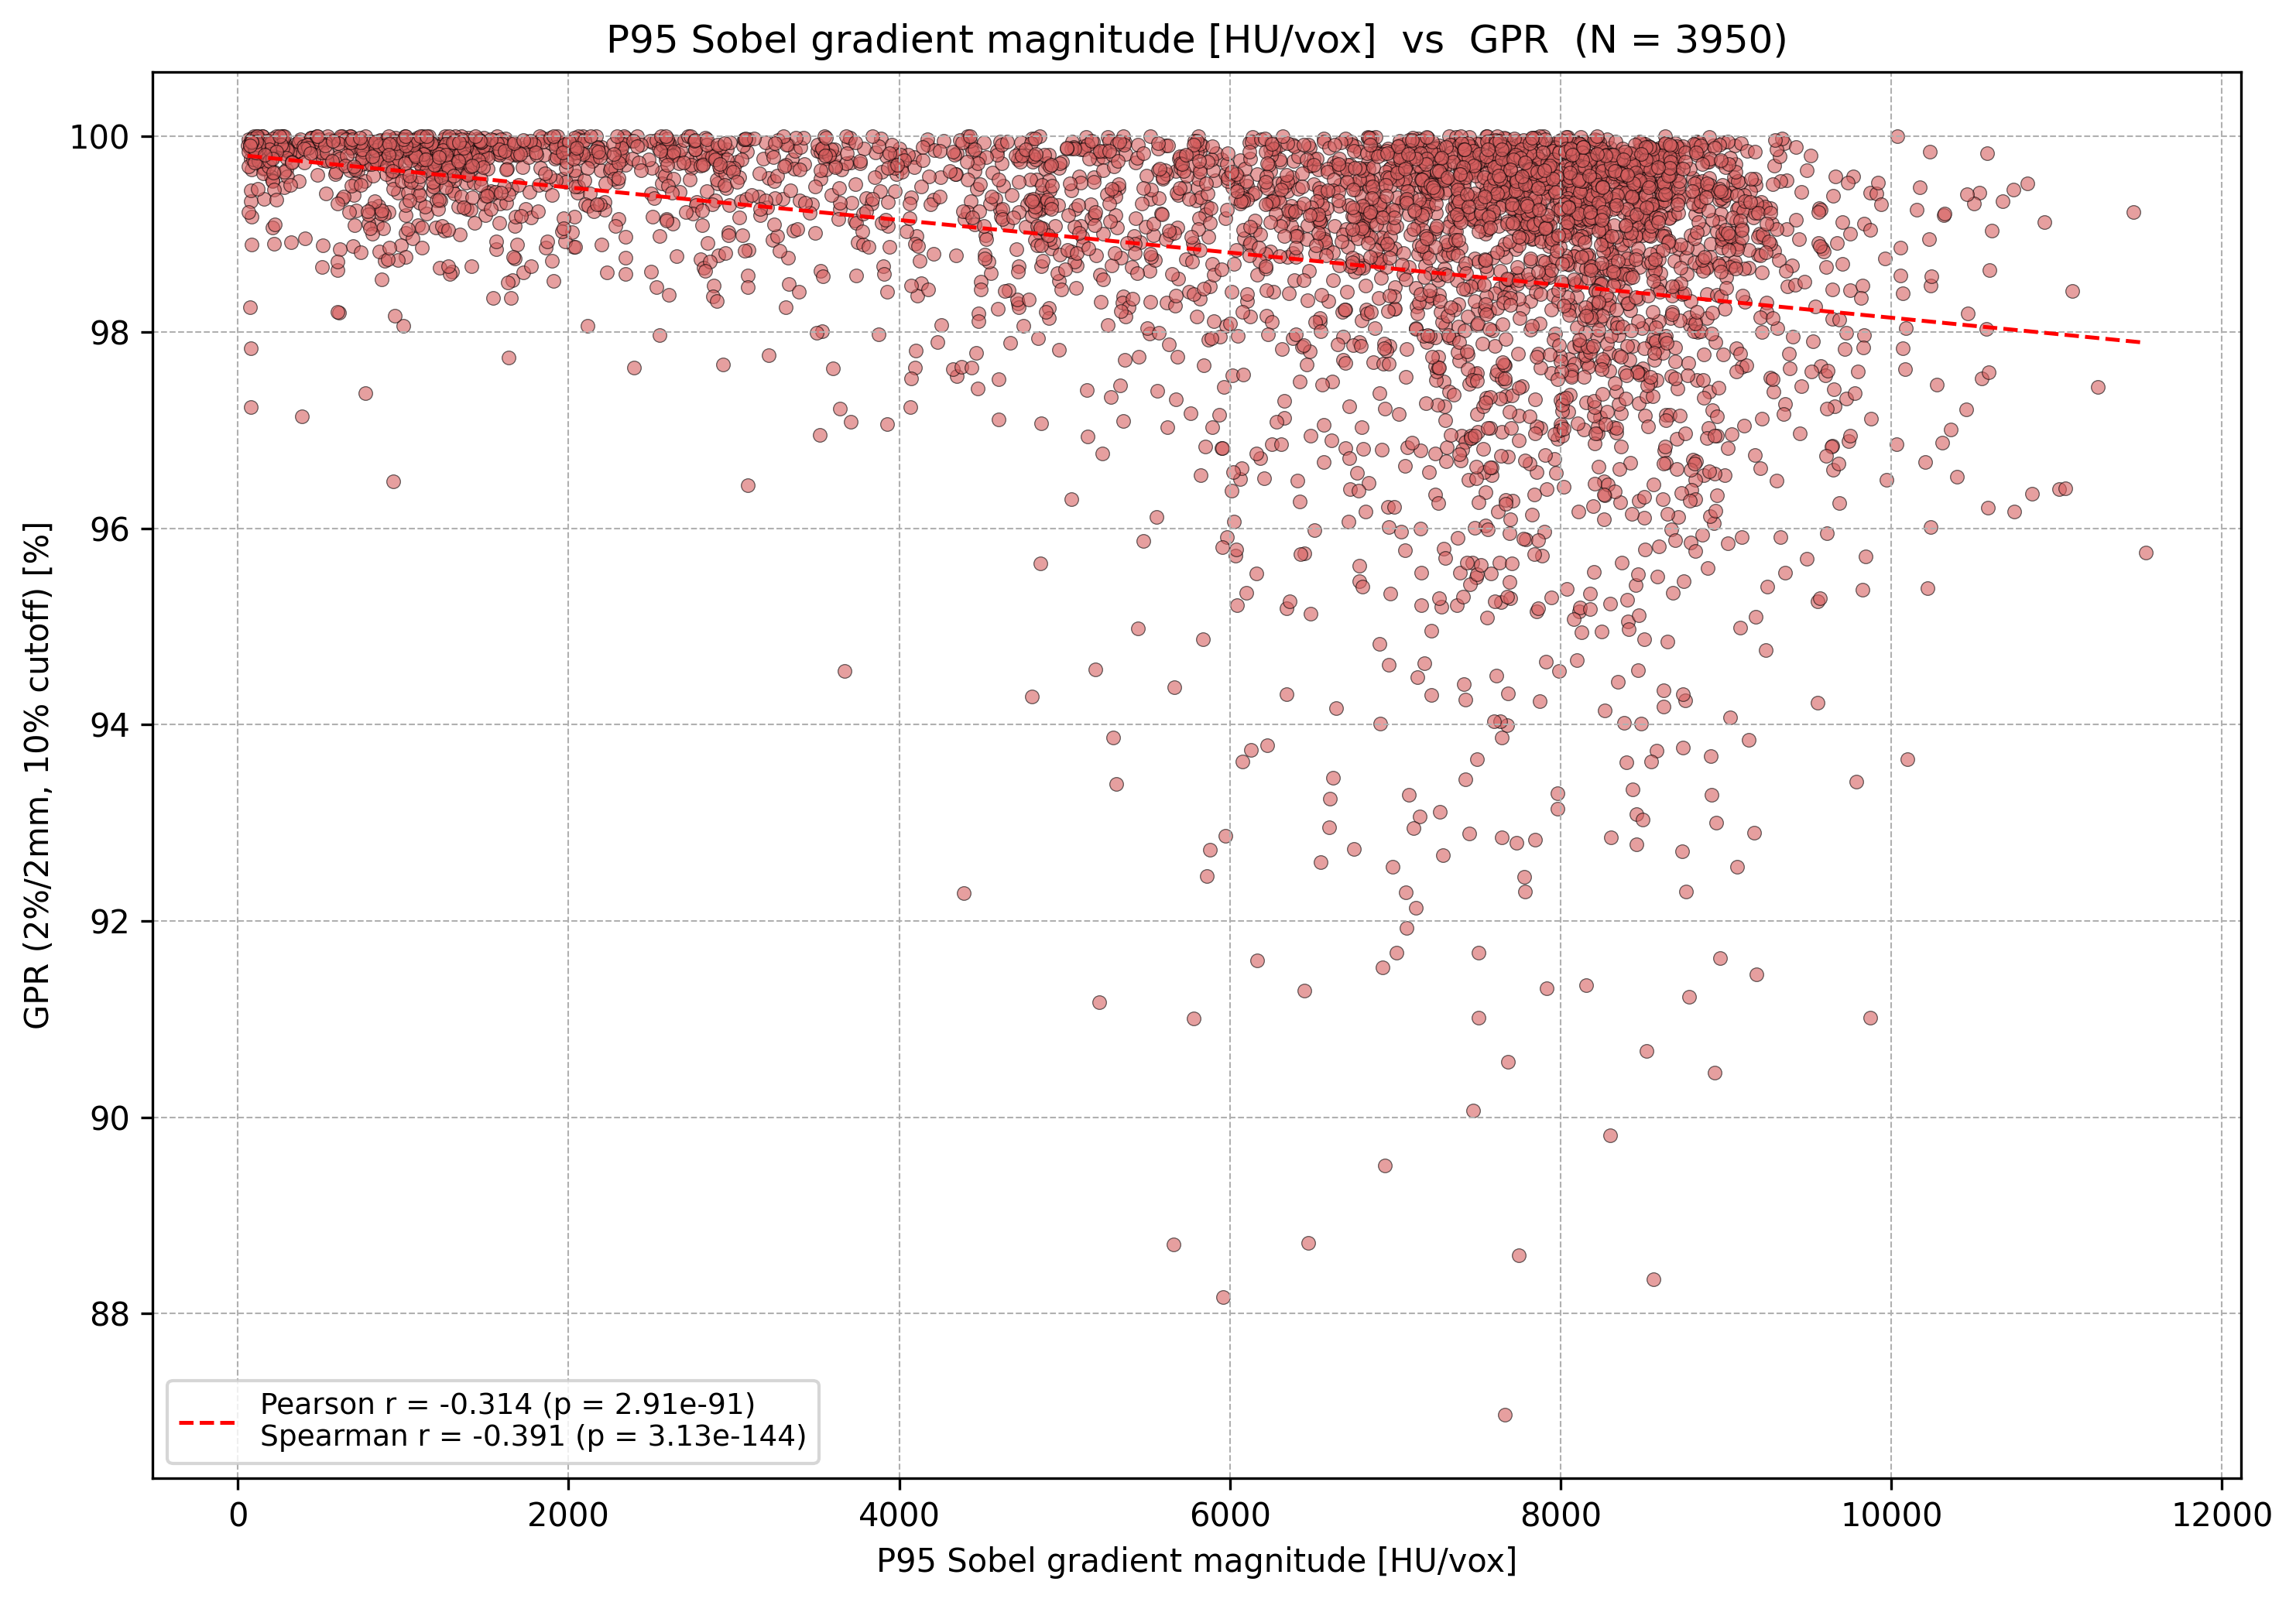
\includegraphics[height=0.72\textheight]{p95_sobel_bp_vs_gpr.png}
  \end{center}
  \vspace{-4pt}
  {\small $S_{95,\text{BP}}$ achieves the strongest correlation with GPR
  (Spearman $\rho = -0.391$). Higher edge responses in the
  BP region are associated with lower gamma pass rates.}
\end{frame}

% ════════════════════════════════════════════════════════════
\section{Energy-Stratified Analysis}
% ════════════════════════════════════════════════════════════

\begin{frame}{Motivation for Energy Stratification}
  \textbf{Observation}: beam energy influences both the anatomy traversed
  and the model's prediction difficulty.

  \vspace{6pt}
  \textbf{Question}: are the observed correlations genuine reflections of
  tissue heterogeneity, or are they confounded by energy?

  \vspace{8pt}
  \textbf{Three complementary analyses:}
  \begin{enumerate}
    \item \textbf{Binned correlations}: compute Spearman $\rho$ within each
          \SI{30}{MeV} energy bin independently.
    \item \textbf{Energy-coloured scatter plots}: visualise metric vs GPR
          with colour encoding beam energy.
    \item \textbf{Partial correlations}: compute partial Spearman
          correlation controlling for energy:
          \begin{equation*}
            \rho_{XY \cdot Z} = \frac{\rho_{XY} - \rho_{XZ}\,\rho_{YZ}}
            {\sqrt{(1 - \rho_{XZ}^2)(1 - \rho_{YZ}^2)}}
          \end{equation*}
          where $X$ = metric, $Y$ = GPR, $Z$ = energy.
  \end{enumerate}
\end{frame}

\begin{frame}{Spearman Correlation by Energy Bin}
  \begin{center}
    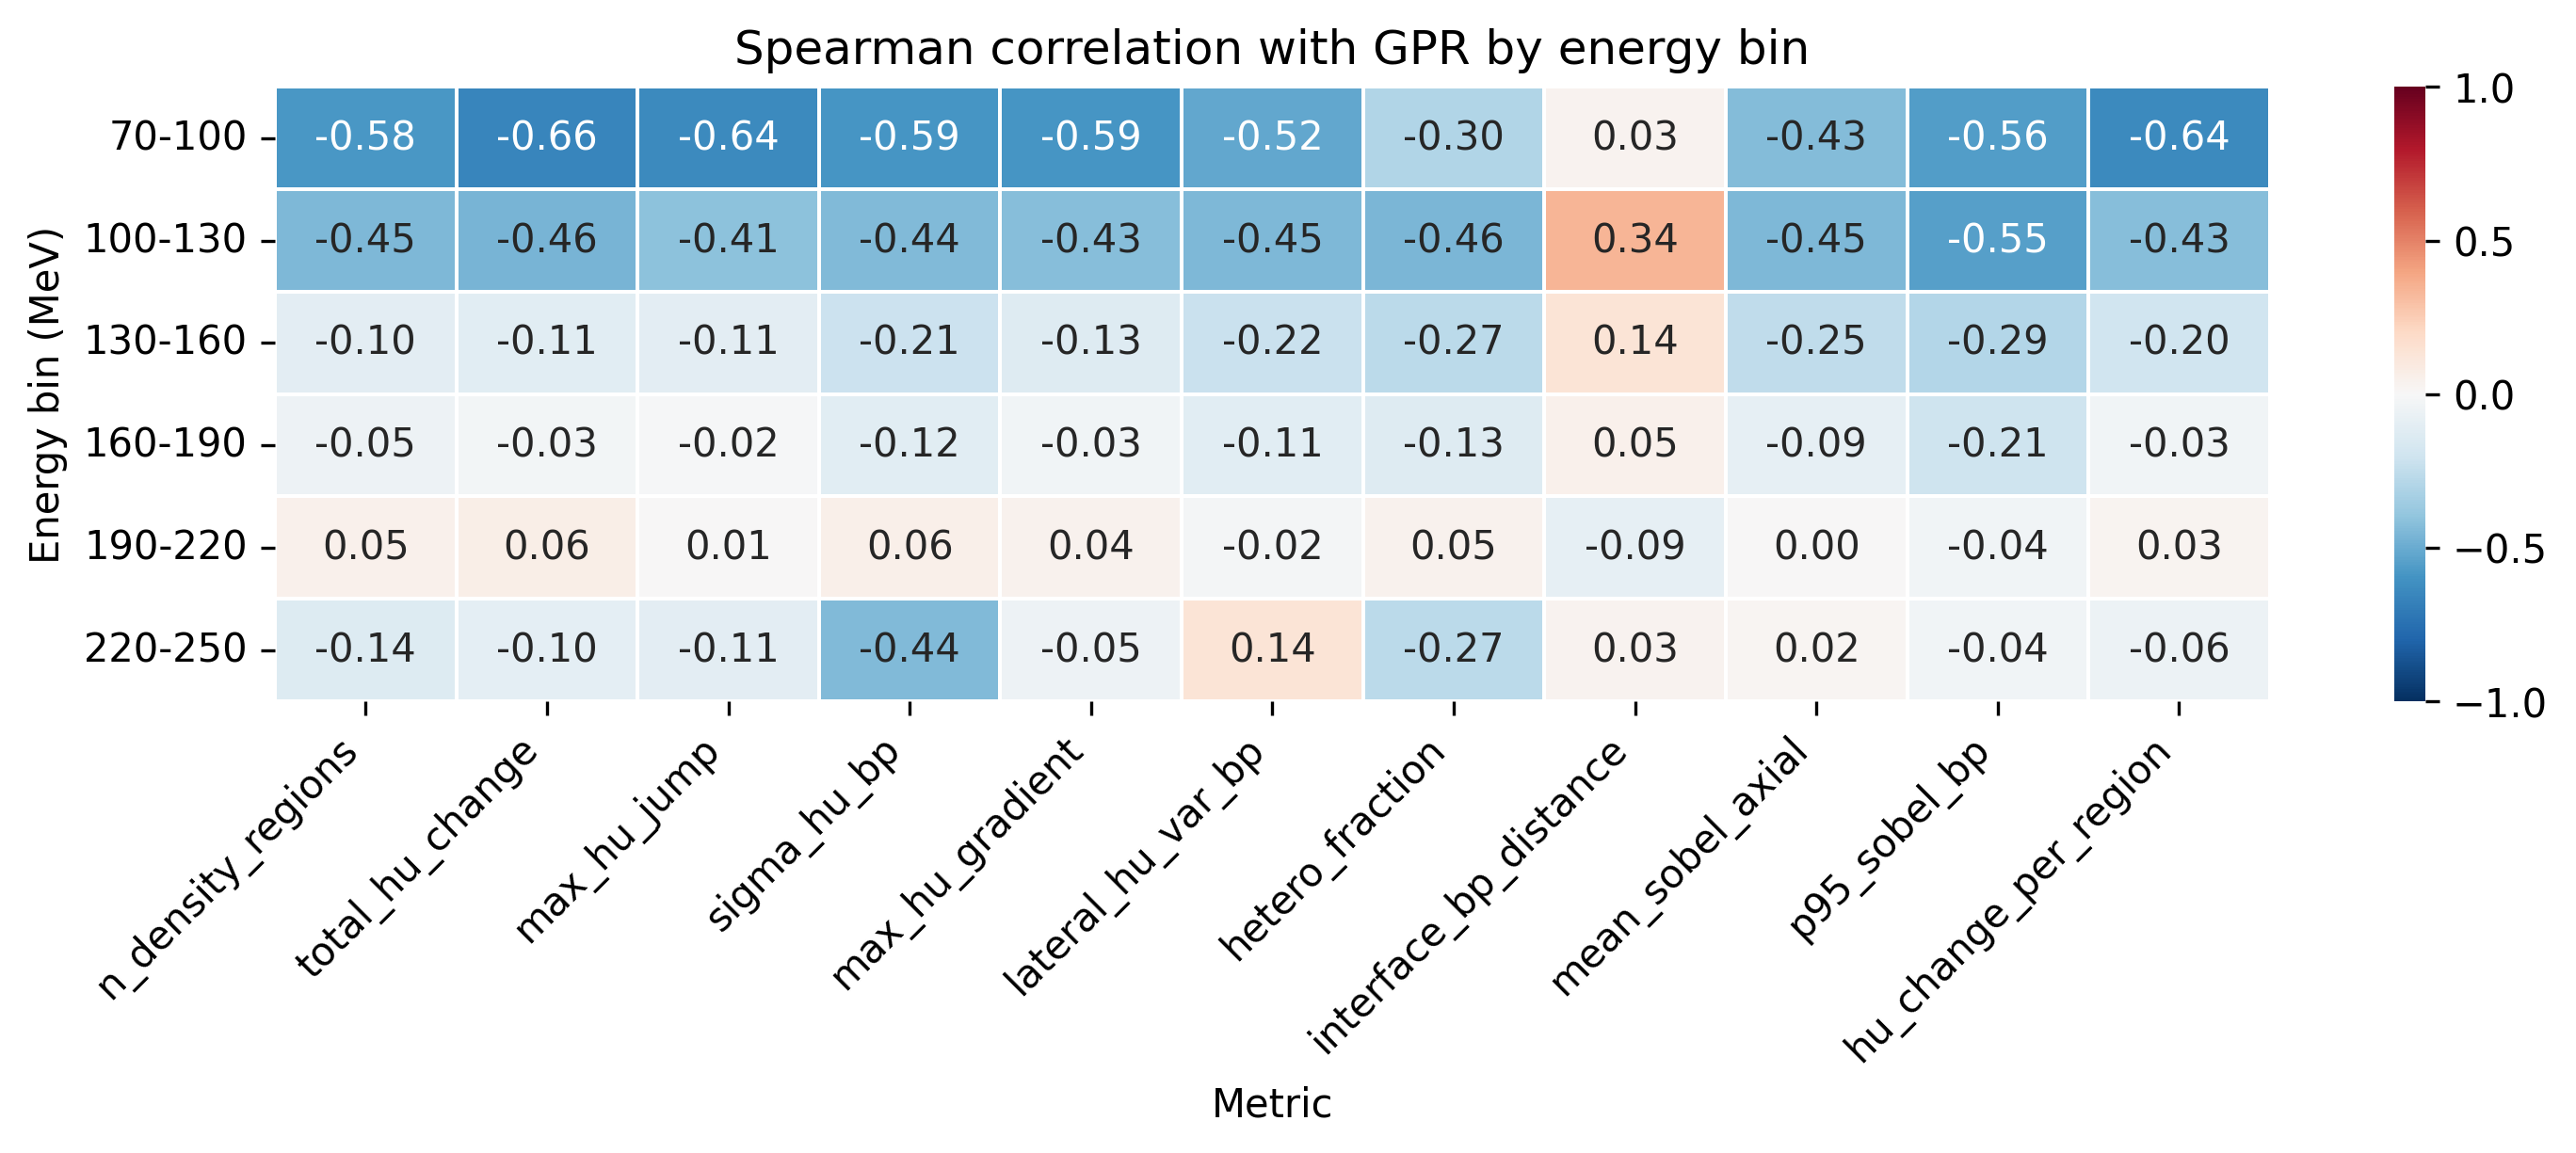
\includegraphics[height=0.78\textheight]{spearman_heatmap_by_energy.png}
  \end{center}
  \vspace{-6pt}
  {\small Correlations are \textbf{strongest at low energies}
  (70--\SI{130}{MeV}: $|\rho| > 0.4$ for top metrics), weaken above
  \SI{160}{MeV}, and largely vanish in the 190--\SI{220}{MeV} bin.}
\end{frame}

\begin{frame}{Energy-Coloured Scatter: P95 Sobel at BP}
  \begin{center}
    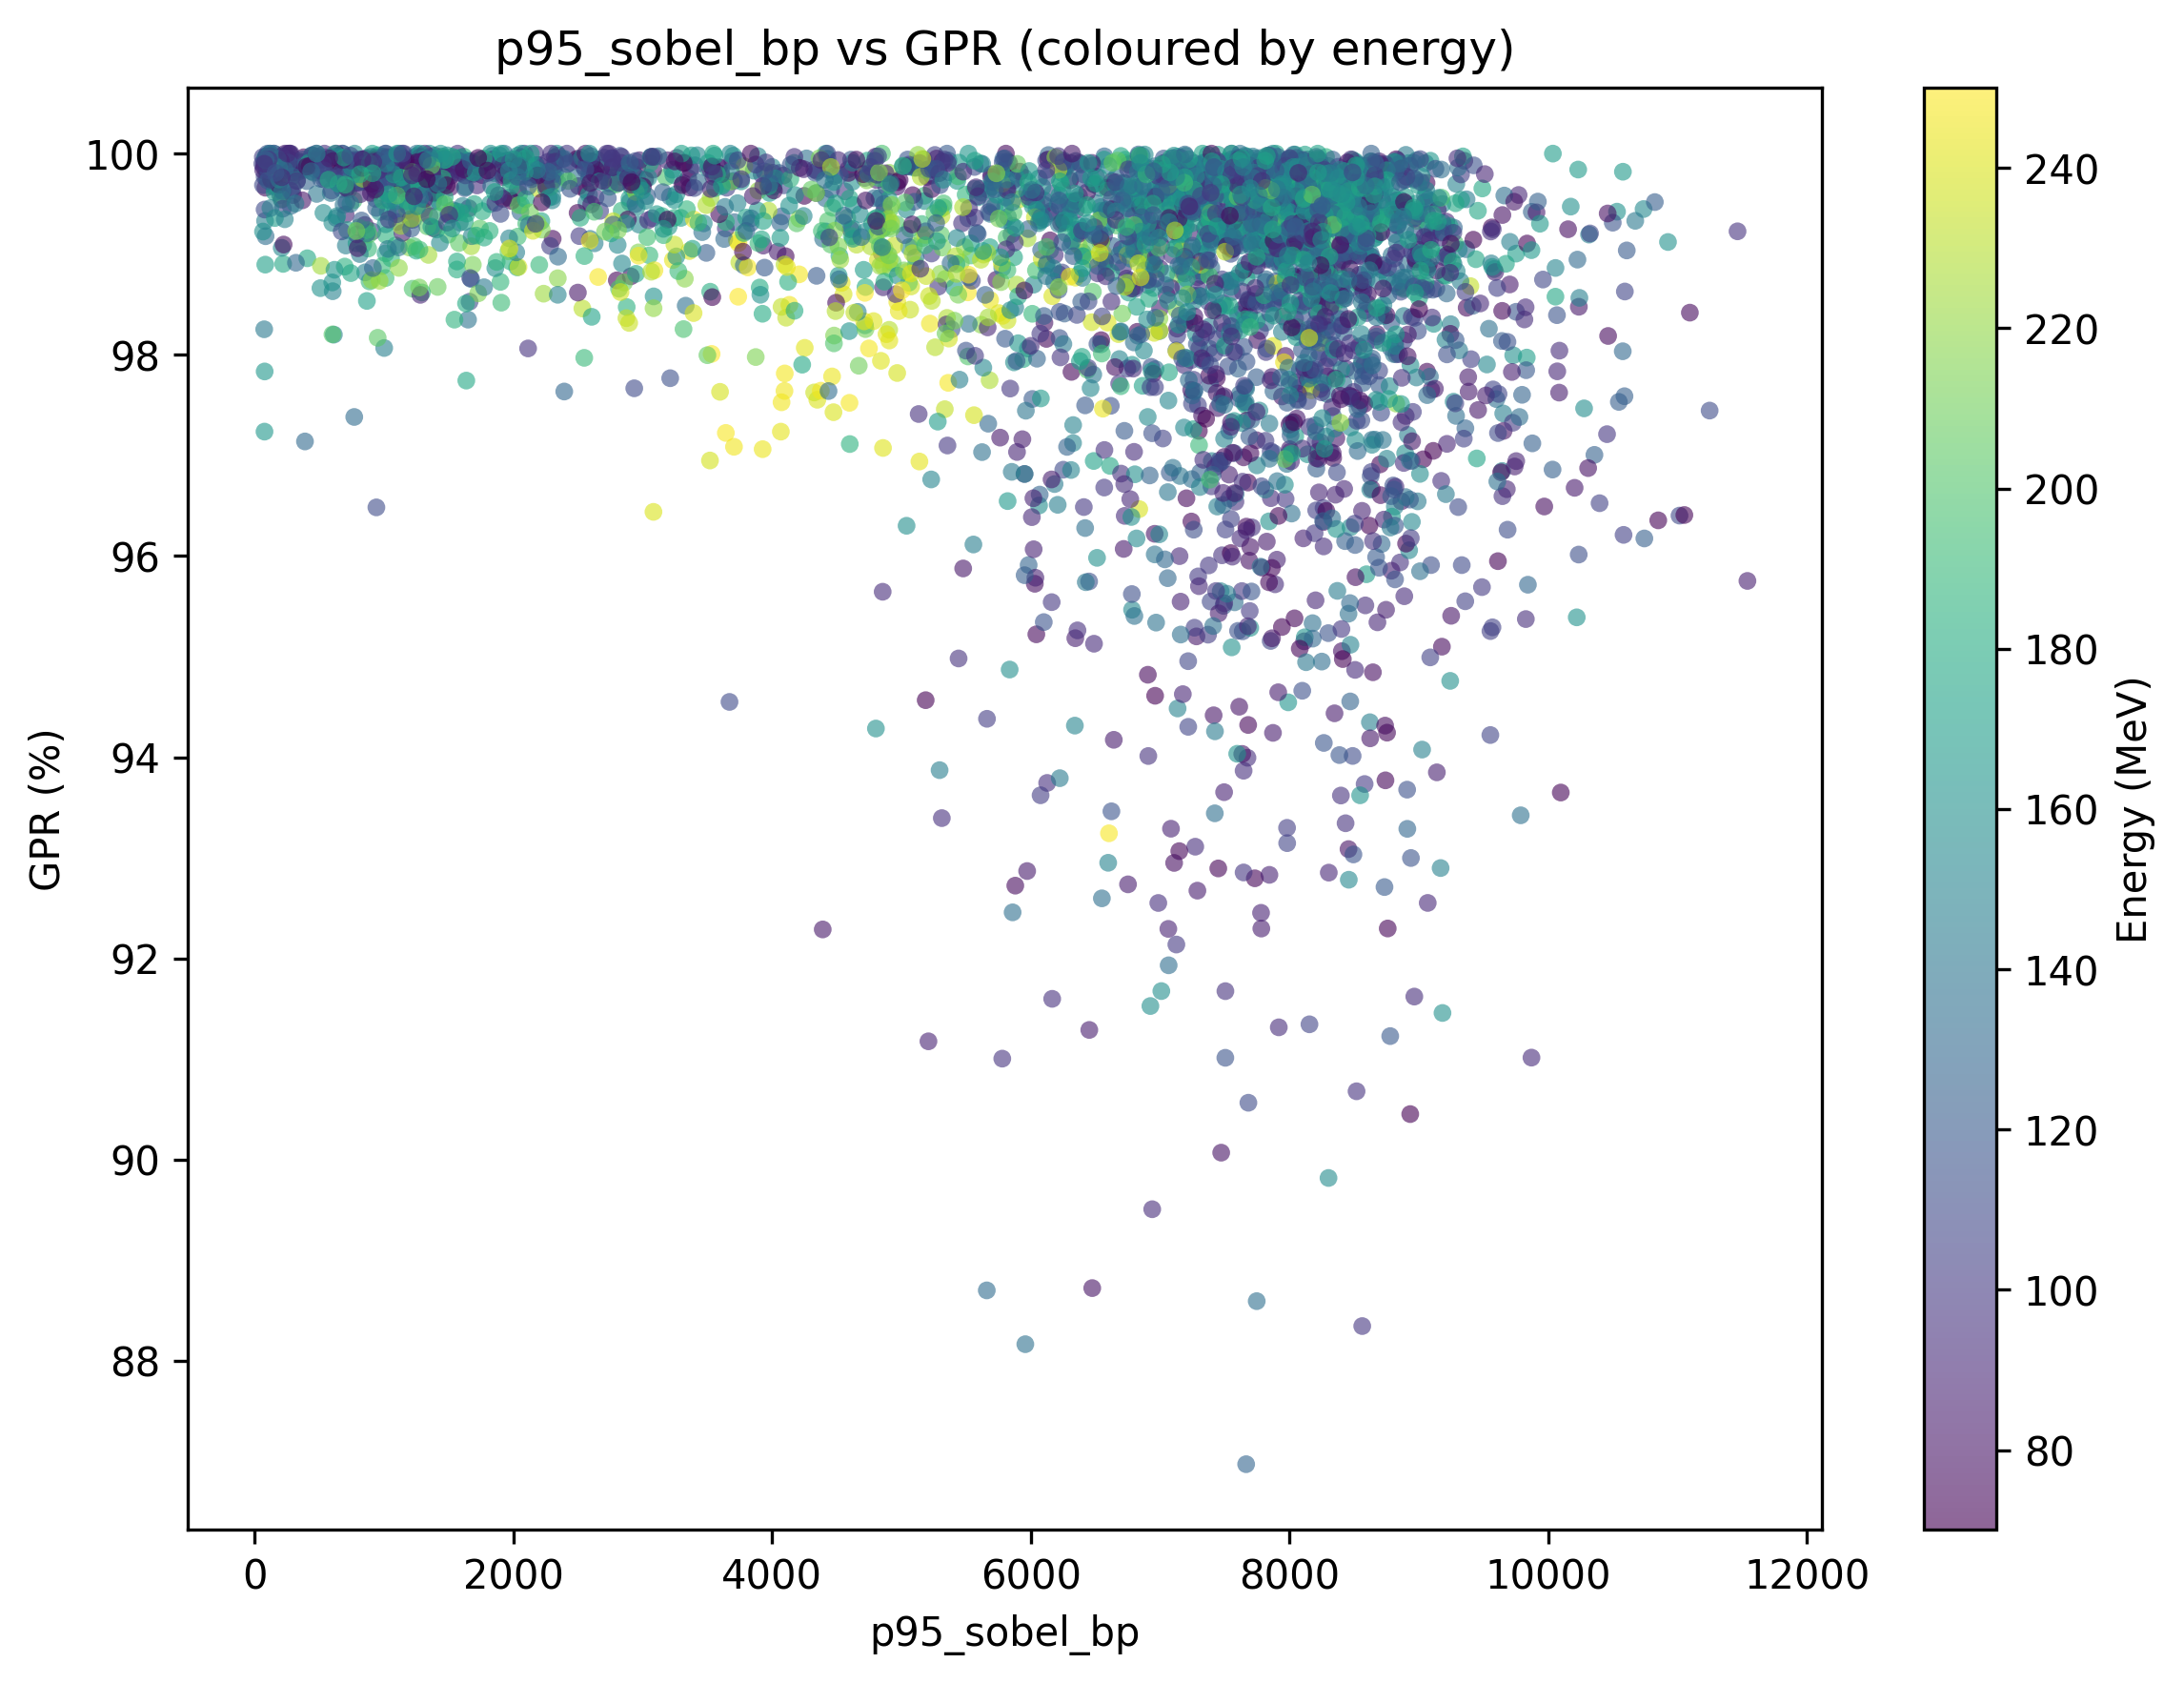
\includegraphics[height=0.78\textheight]{p95_sobel_bp_vs_gpr_energy_coloured.png}
  \end{center}
  \vspace{-6pt}
  {\small Low-energy beamlets (dark) populate the high-$S_{95}$ / low-GPR
  region.  At higher energies the metric range compresses and GPR clusters
  near 99--100\%.}
\end{frame}

\begin{frame}{Partial Correlations Controlling for Energy}
  \begin{columns}[T]
    \begin{column}{0.52\textwidth}
      \vspace{-4pt}
      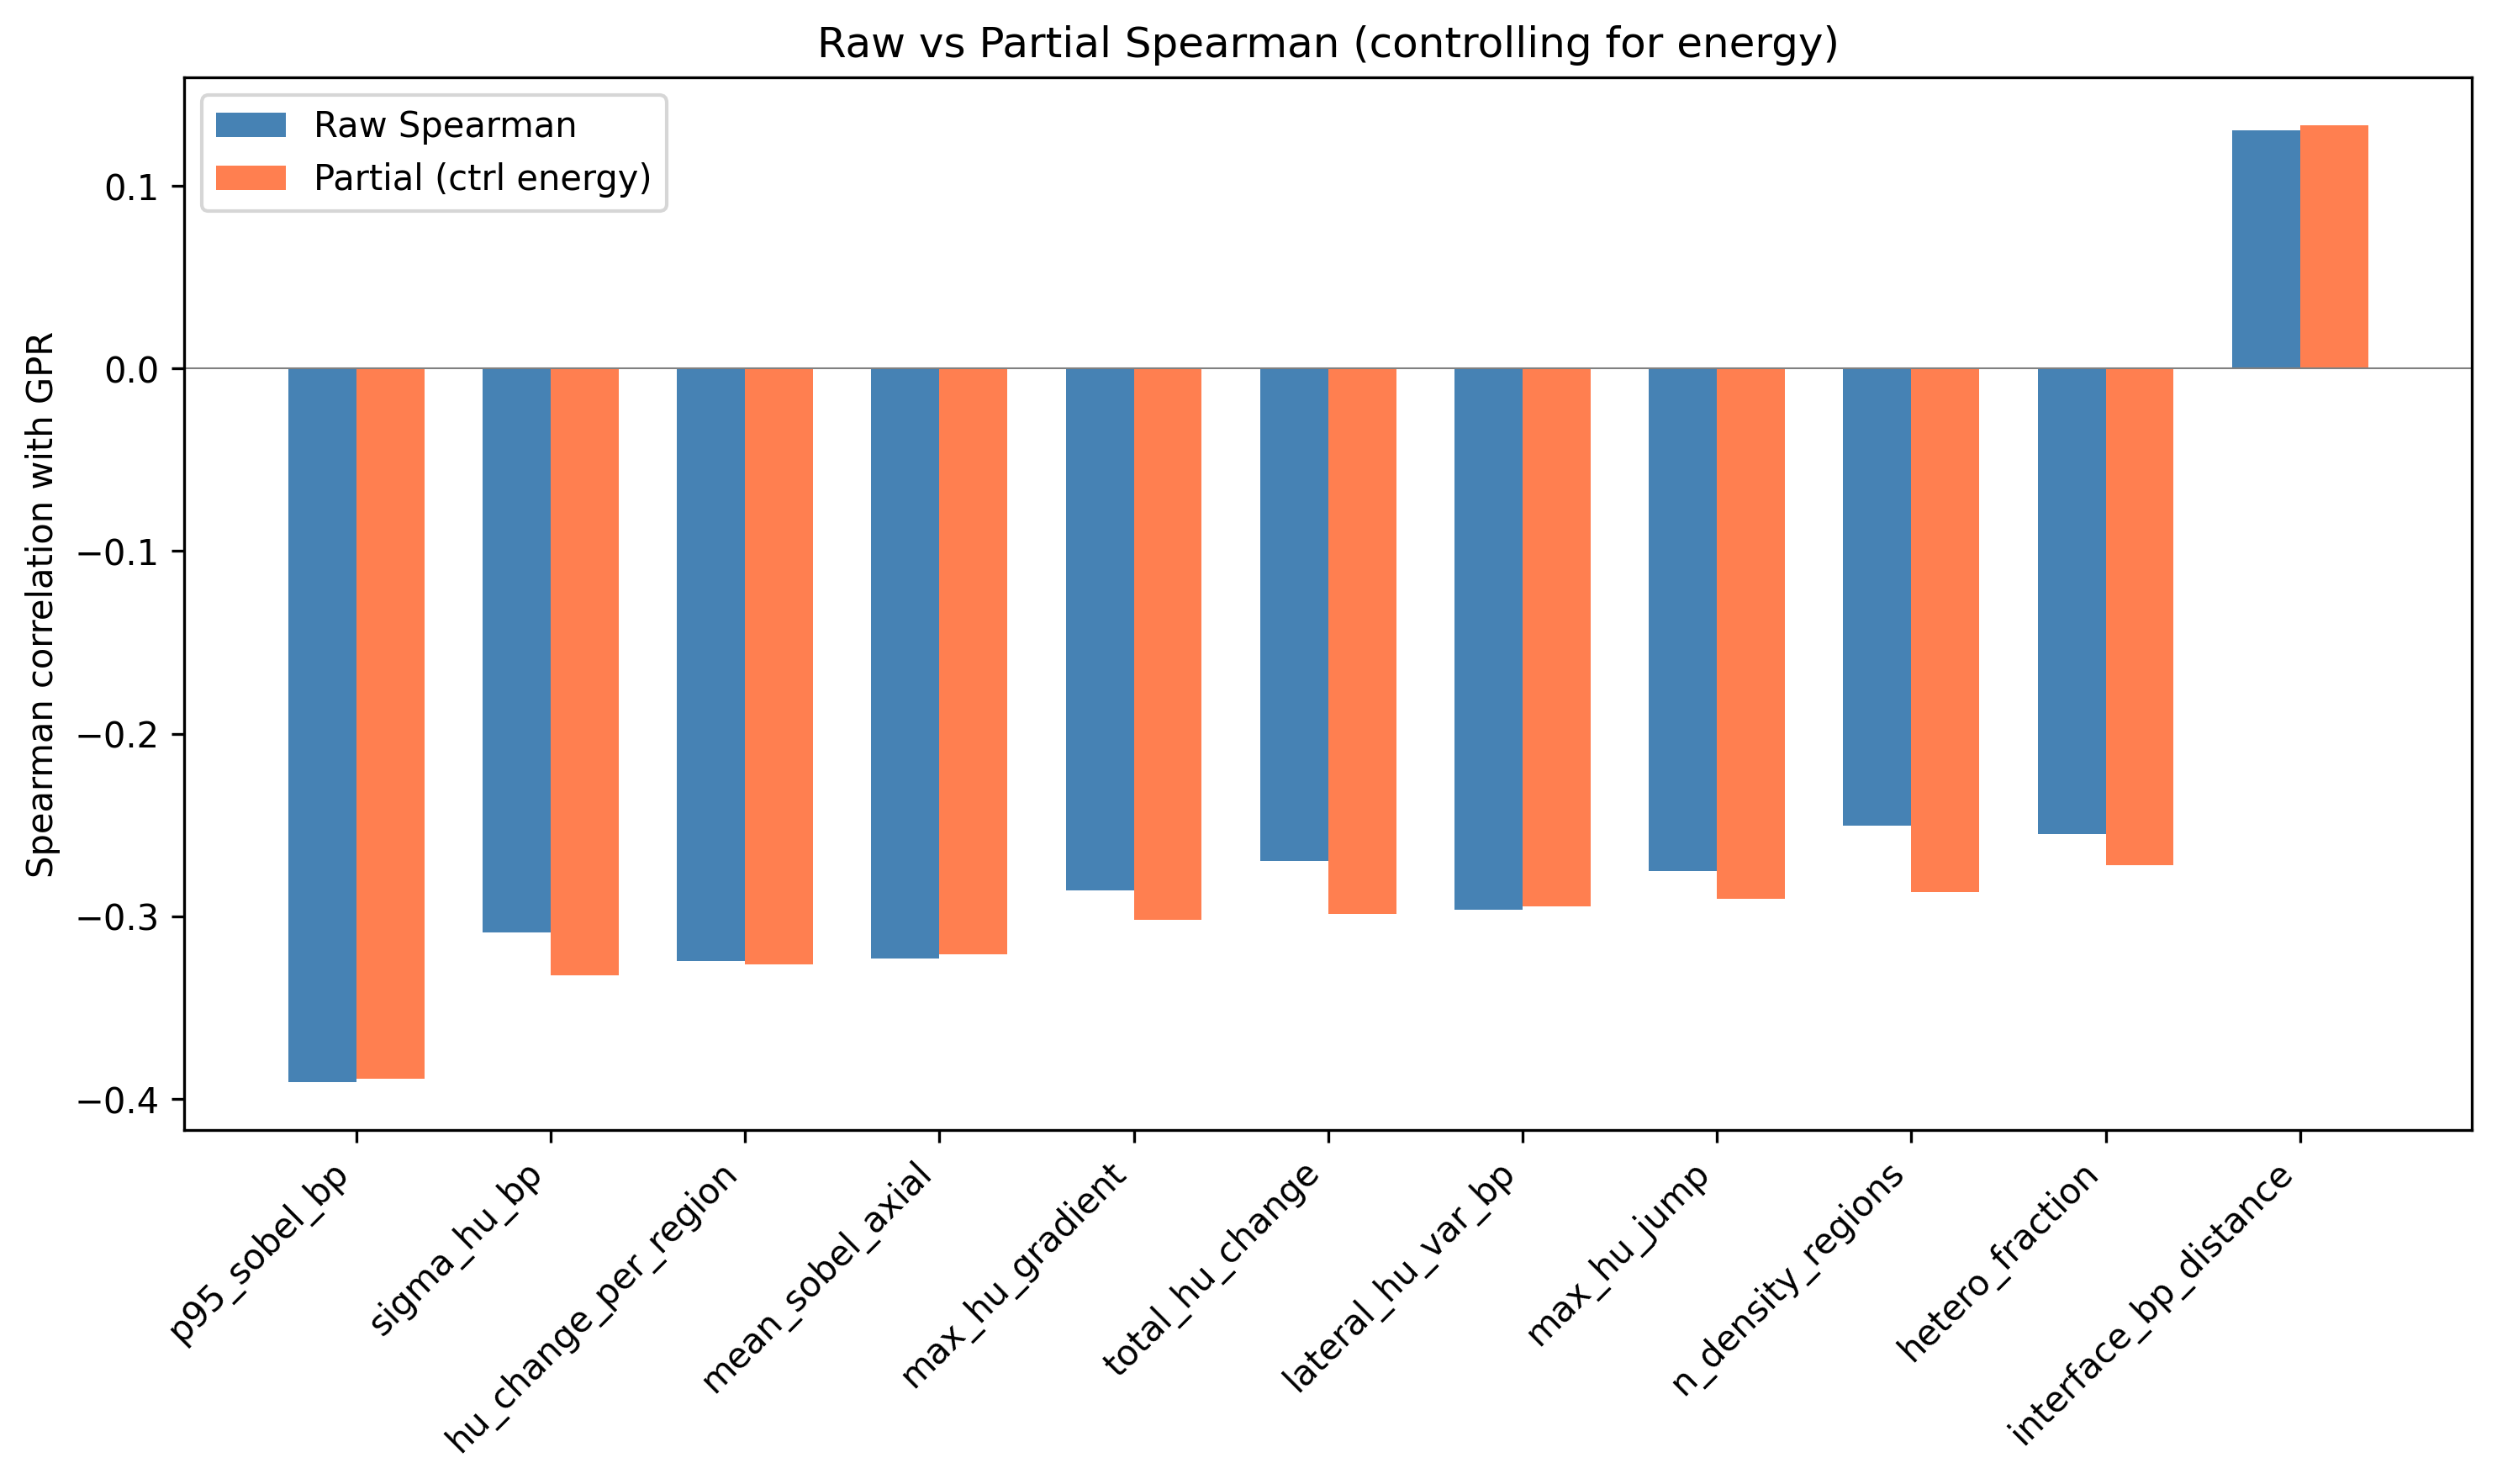
\includegraphics[width=\textwidth]{partial_vs_raw_correlation.png}
    \end{column}
    \begin{column}{0.46\textwidth}
      \vspace{2pt}
      {\small
      \begin{tabular}{lrr}
        \toprule
        \textbf{Metric} & \textbf{Raw} & \textbf{Partial} \\
        \midrule
        p95\_sobel\_bp      & $-0.391$ & $-0.389$ \\
        $\sigma_{\text{HU,BP}}$ & $-0.309$ & $-0.332$ \\
        $\Delta H/n_{\text{reg}}$ & $-0.324$ & $-0.326$ \\
        $\bar{S}_{\text{axial}}$ & $-0.323$ & $-0.321$ \\
        $g_{\max}$          & $-0.286$ & $-0.302$ \\
        $n_{\text{regions}}$ & $-0.251$ & $-0.287$ \\
        \bottomrule
      \end{tabular}
      }

      \vspace{6pt}
      {\small Raw and partial correlations differ by $|\Delta| < 0.04$:
      heterogeneity--GPR associations are \textbf{not confounded by energy}.
      For $n_{\text{regions}}$ ($\Delta = -0.036$), controlling for energy
      \emph{strengthens} the correlation.}
    \end{column}
  \end{columns}
\end{frame}

% ════════════════════════════════════════════════════════════
\section{Discussion \& Key Findings}
% ════════════════════════════════════════════════════════════

\begin{frame}{Key Findings}
  \begin{enumerate}
    \item \textbf{P95 Sobel at BP is the strongest single predictor} of GPR
          degradation ($\rho_s = -0.391$), capturing sharp density
          transitions near the Bragg peak via gradient-based edge detection.

    \vspace{6pt}
    \item \textbf{Spearman $\gg$ Pearson} for most metrics, indicating
          \textbf{monotonic but non-linear} relationships between tissue
          heterogeneity and prediction difficulty.

    \vspace{6pt}
    \item \textbf{Correlations are energy-dependent}: strongest at low
          energies (70--\SI{130}{MeV}, $|\rho_s|$ up to $0.66$), weak to
          absent above \SI{160}{MeV}.
          \begin{itemize}
            \item Low-energy beams have shorter ranges $\rightarrow$ tissue
                  heterogeneity has proportionally larger impact.
            \item High-energy beams traverse more uniform deep tissue.
          \end{itemize}

    \vspace{6pt}
    \item \textbf{Partial correlations confirm}: energy is \emph{not} a
          confounder: the heterogeneity--GPR association persists after
          controlling for beam energy ($|\Delta\rho| < 0.04$).
  \end{enumerate}
\end{frame}

% ════════════════════════════════════════════════════════════
\section{Proposed: VLM-based Difficulty Estimation}
% ════════════════════════════════════════════════════════════

% ── Motivation ──────────────────────────────────────────────
\begin{frame}{Motivation: Beyond Handcrafted Metrics}
  \textbf{Current status}: best single predictor ($S_{95,\text{BP}}$)
  reaches only $|\rho_s| \approx 0.39$.

  \vspace{6pt}
  \textbf{Key insight from Jungo et~al.~(2020)}~\cite{jungo2020}:
  voxel-wise uncertainty is unreliable, but \emph{subject-level aggregated}
  features accurately detect segmentation failures (AUC-ROC $> 0.85$).

  \vspace{6pt}
  \textbf{Idea}: replace manual feature engineering with a
  Vision-Language Model (VLM) that performs implicit visual aggregation
  over the beamlet geometry.

  \vspace{8pt}
  \begin{block}{Core hypothesis}
    A VLM can capture richer spatial patterns (irregular bone-tissue
    interfaces, air cavities, complex anatomy near the beam path)
    than any single scalar metric, yielding a stronger and more
    \emph{reproducible} difficulty score.
  \end{block}
\end{frame}

% ── Pipeline overview ───────────────────────────────────────
\begin{frame}{Proposed Pipeline: Overview}
  \centering
  \vspace{-2pt}
  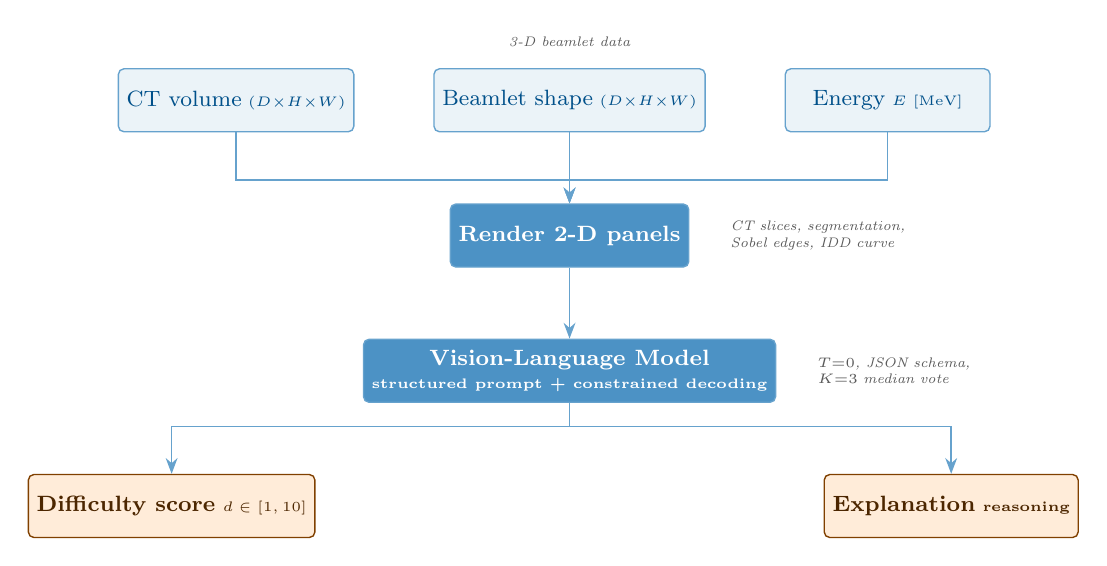
\begin{tikzpicture}[
      node distance=4mm and 10mm,
      every node/.style={font=\footnotesize},
      box/.style={draw=tudelft!60, rounded corners=2pt, line width=0.5pt,
                  minimum height=8mm, minimum width=26mm, align=center,
                  inner sep=3pt},
      inp/.style={box, fill=tudelft!8, text=tudelft!80!black},
      proc/.style={box, fill=tudelft!70, text=white,
                   font=\footnotesize\bfseries},
      outp/.style={box, fill=orange!15, draw=orange!50!black,
                   text=orange!30!black, font=\footnotesize\bfseries},
      arr/.style={-{Stealth[length=2mm, width=1.5mm]}, semithick,
                  color=tudelft!60},
      lbl/.style={font=\tiny\itshape, text=gray!70!black},
    ]
    % ── Row 1: Inputs ───────────────────────────────────────
    \node[inp] (ct)   {CT volume\;{\tiny$(D{\times}H{\times}W)$}};
    \node[inp, right=10mm of ct] (flux)
      {Beamlet shape\;{\tiny$(D{\times}H{\times}W)$}};
    \node[inp, right=10mm of flux] (eng)
      {Energy\;{\tiny$E$ [MeV]}};

    \node[lbl, above=1.5mm of flux] {3-D beamlet data};

    % ── Row 2: Rendering ────────────────────────────────────
    \node[proc, below=9mm of flux] (render)
      {Render 2-D panels};
    \node[lbl, right=4mm of render.east, text width=26mm]
      {CT slices, segmentation,\\Sobel edges, IDD curve};

    % ── Row 3: VLM ──────────────────────────────────────────
    \node[proc, below=9mm of render, minimum width=34mm] (vlm)
      {Vision-Language Model\\[-1pt]{\tiny\color{white!80}%
       structured prompt + constrained decoding}};
    \node[lbl, right=4mm of vlm.east, text width=26mm]
      {$T{=}0$, JSON schema,\\$K{=}3$ median vote};

    % ── Row 4: Outputs ──────────────────────────────────────
    \node[outp, below left=9mm and 6mm of vlm] (score)
      {Difficulty score\;{\tiny$d \in [1,10]$}};
    \node[outp, below right=9mm and 6mm of vlm] (expl)
      {Explanation\;{\tiny reasoning}};

    % ── Arrows ──────────────────────────────────────────────
    \draw[arr] (ct.south)   |- ([yshift=3mm]render.north) -- (render.north);
    \draw[arr] (flux.south) -- (render.north);
    \draw[arr] (eng.south)  |- ([yshift=3mm]render.north) -- (render.north);
    \draw[arr] (render.south) -- (vlm.north);
    \draw[arr] (vlm.south) -- ++(0,-3mm) -| (score.north);
    \draw[arr] (vlm.south) -- ++(0,-3mm) -| (expl.north);
  \end{tikzpicture}
\end{frame}

% ── Input specification ─────────────────────────────────────
\begin{frame}{Input Specification}
  The VLM receives a \textbf{structured prompt} composed of:

  \vspace{2pt}
  \begin{columns}[T]
    \begin{column}{0.52\textwidth}
      \textbf{1.\ Image panel} (rendered from 3-D data):
      \begin{itemize}\setlength{\itemsep}{1pt}
        \item Axial \& coronal CT slices at BP depth
        \item 7-class tissue segmentation overlay
        \item Sobel edge-magnitude map (hot colourmap)
        \item IDD curve with BP range annotation
        \item Beamlet-shape projection (flux) overlay
      \end{itemize}
    \end{column}
    \begin{column}{0.44\textwidth}
      \textbf{2.\ Text metadata}:
      \begin{itemize}\setlength{\itemsep}{1pt}
        \item Initial beam energy $E$ [MeV]
        \item BP depth range $[z_{\min}, z_{\max}]$ [mm]
        \item Number of density regions $n_{\text{reg}}$
        \item Voxel resolution [\SI{}{mm}]
      \end{itemize}

      \vspace{4pt}
      {\footnotesize\textbf{Note}: reuses the existing
      \texttt{plot\_ct\_with\_segmentation} figures.}
    \end{column}
  \end{columns}

  \vspace{4pt}
  \begin{alertblock}{\footnotesize Limitation: ground-truth dependency}
    {\footnotesize The current pipeline relies on \textbf{ground-truth dose}
    (MC) for BP range estimation, IDD rendering, and GPR labels,
    so it is not yet applicable in an \textbf{active learning} setting.
    Future work: replace GT-derived features with CT-only surrogates.}
  \end{alertblock}
\end{frame}

% ── Scoring: reproducibility ───────────────────────────────
\begin{frame}{Reproducible Difficulty Scoring}
  \textbf{Critical requirement}: the scoring pipeline must be
  \emph{deterministic and reproducible}.

  \vspace{6pt}
  \textbf{Strategy}: structured output with constrained decoding.

  \vspace{4pt}
  \begin{enumerate}
    \item Set VLM temperature $T = 0$ (greedy decoding) to eliminate
          sampling randomness.
    \item Use a JSON-schema-constrained output format
          (supported by OpenAI, vLLM, Outlines~\cite{willard2023}):
          \vspace{2pt}
          {\small\texttt{\{"difficulty": int, "confidence": float,
          "reason": str\}}}
    \item Run $K{=}3$ independent forward passes per beamlet;
          report \textbf{median} score and inter-run agreement
          ($\kappa$) as a built-in reliability check.
    \item Validate against held-out GPR ground truth with
          Spearman $\rho$ and failure-detection AUC-ROC
          (following Jungo et~al.~\cite{jungo2020}).
  \end{enumerate}

  \vspace{4pt}
  {\small With constrained decoding and $T{=}0$, identical inputs
  produce identical outputs on the same model checkpoint.}
\end{frame}

% ── Experimental tracks ─────────────────────────────────────
\begin{frame}{Experimental Tracks}
  \begin{center}
  \renewcommand{\arraystretch}{1.3}
  {\small
  \begin{tabular}{@{}l l l l@{}}
    \toprule
    \textbf{Track} & \textbf{Method} & \textbf{VLM input} & \textbf{Output} \\
    \midrule
    A & Zero-shot  & Image + metadata prompt
      & Difficulty 1--10 \\
    B & Few-shot   & Same + 5--10 labelled examples
      & Predicted GPR \\
    C & Fine-tuned & LoRA adapter on VLM encoder
      & GPR (continuous) \\
    \bottomrule
  \end{tabular}
  }
  \end{center}

  \vspace{6pt}
  \textbf{Track A} tests whether a general-purpose VLM can reason about
  dose-prediction difficulty \emph{without any training}.

  \textbf{Track B} adds in-context learning with a handful of extreme
  cases (best/worst GPR) as calibration anchors.

  \textbf{Track C} fine-tunes a lightweight adapter (LoRA,
  Hu et~al.~\cite{hu2022lora}) on the $n{=}3\,950$ dataset, mapping
  VLM visual features directly to continuous GPR.

  \vspace{4pt}
  {\small Evaluation: Spearman/Pearson $\rho$ vs.\ actual GPR,
  AUC-ROC for failure detection (GPR $< 95\%$), energy-stratified
  breakdown.}
\end{frame}

% ── Computational cost ──────────────────────────────────────
\begin{frame}{Computational Cost Analysis}
  \textbf{Constraint}: VLM scoring must be \emph{significantly cheaper}
  than Monte Carlo simulation.

  \vspace{6pt}
  \begin{center}
  \renewcommand{\arraystretch}{1.3}
  {\small
  \begin{tabular}{@{}l r r r@{}}
    \toprule
    \textbf{Method} & \textbf{Time/beamlet} & \textbf{GPU} \\
    \midrule
    MC simulation (TOPAS)
      & $\sim$\SI{60}{s}  & none (CPU cluster)  \\
    ADoTA inference
      & \SI{1.7}{ms}      & 1$\times$ consumer GPU   \\
    VLM Track A (API)
      & $\sim$\SI{2}{s}   & none (cloud)       \\
    VLM Track C (local, 7B)
      & $\sim$\SI{0.3}{s} & 1$\times$ A100     \\
    \bottomrule
  \end{tabular}
  }
  \end{center}

  \vspace{6pt}
  \begin{itemize}
    \item API-based Track A/B: ${\sim}50\times$ cheaper than MC.
    \item Local 7B model (Track C): ${\sim}200\times$ cheaper than MC,
          and all computation stays on-premise (data privacy).
    \item Full training plan with $n{=}3\,950$: a single LoRA
          fine-tuning epoch on a 7B VLM takes ${\sim}$\SI{15}{min}
          on one A100 (Liu et~al.~\cite{liu2024visual}).
  \end{itemize}
\end{frame}

% ── Architecture diagram: Track C ──────────────────────────
\begin{frame}{Track C: Fine-tuned VLM Architecture}
  \centering
  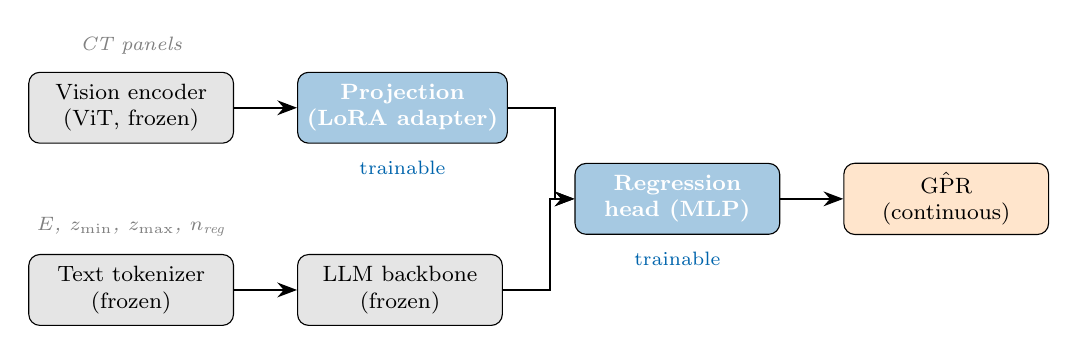
\begin{tikzpicture}[
      node distance=7mm and 8mm,
      box/.style={draw, rounded corners, minimum height=9mm,
                  minimum width=26mm, align=center, font=\footnotesize},
      frozen/.style={box, fill=gray!20},
      train/.style={box, fill=tudelft!35, text=white,
                    font=\footnotesize\bfseries},
      outp/.style={box, fill=orange!20},
      arr/.style={-{Stealth[length=2.5mm]}, thick},
    ]
    % Image path
    \node[frozen]                         (vit)   {Vision encoder\\(ViT, frozen)};
    \node[train, right=of vit]            (proj)  {Projection\\(LoRA adapter)};

    % Text path
    \node[frozen, below=14mm of vit]      (tok)   {Text tokenizer\\(frozen)};
    \node[frozen, right=of tok]           (llm)   {LLM backbone\\(frozen)};

    % Fusion + head
    \node[train, right=22mm of $(proj)!0.5!(llm)$] (head) {Regression\\head (MLP)};
    \node[outp, right=of head]             (gpr)   {$\hat{\text{GPR}}$\\(continuous)};

    % Arrows
    \draw[arr] (vit)  -- (proj);
    \draw[arr] (proj.east) -- ++(6mm,0) |- (head);
    \draw[arr] (tok)  -- (llm);
    \draw[arr] (llm.east) -- ++(6mm,0) |- (head);
    \draw[arr] (head) -- (gpr);

    % Labels
    \node[above=1mm of vit, font=\scriptsize\itshape, text=gray]
      {CT panels};
    \node[above=1mm of tok, font=\scriptsize\itshape, text=gray]
      {$E$, $z_{\min}$, $z_{\max}$, $n_{\text{reg}}$};
    \node[below=1mm of proj, font=\scriptsize, text=tudelft]
      {trainable};
    \node[below=1mm of head, font=\scriptsize, text=tudelft]
      {trainable};
  \end{tikzpicture}

  \vspace{6pt}
  {\small Only the LoRA projection and the regression head are trained
  (${\sim}$2--4\,M parameters).  Vision encoder and LLM backbone stay
  frozen, making fine-tuning feasible on a single GPU.

  \vspace{2pt}
  Candidate models: LLaVA-1.5-7B~\cite{liu2024visual},
  Qwen2-VL-7B~\cite{wang2024qwen2vl}, or BiomedCLIP~\cite{zhang2024biomedclip}
  (if a medical-domain prior is desired).}
\end{frame}

% ── References for VLM section ─────────────────────────────
\begin{frame}{References}
  \small
  \begin{thebibliography}{9}
    \bibitem{jungo2020}
    A.~Jungo, F.~Balsiger, M.~Reyes,
    ``Analyzing the Quality and Challenges of Uncertainty Estimations
    for Brain Tumor Segmentation,''
    \textit{Front.\ Neurosci.}, vol.~14, p.~282, 2020.\\
    \url{https://doi.org/10.3389/fnins.2020.00282}

    \bibitem{willard2023}
    B.~T.~Willard, R.~Louf,
    ``Efficient Guided Generation for Large Language Models,''
    \textit{arXiv:2307.09702}, 2023.\\
    \url{https://arxiv.org/abs/2307.09702}

    \bibitem{hu2022lora}
    E.~J.~Hu et~al.,
    ``LoRA: Low-Rank Adaptation of Large Language Models,''
    \textit{ICLR}, 2022.\\
    \url{https://arxiv.org/abs/2106.09685}

    \bibitem{liu2024visual}
    H.~Liu et~al.,
    ``Visual Instruction Tuning,''
    \textit{NeurIPS}, 2023 (LLaVA).\\
    \url{https://arxiv.org/abs/2304.08485}

    \bibitem{wang2024qwen2vl}
    P.~Wang et~al.,
    ``Qwen2-VL: Enhancing Vision-Language Model's Perception of the World
    at Any Resolution,''
    \textit{arXiv:2409.12191}, 2024.\\
    \url{https://arxiv.org/abs/2409.12191}

    \bibitem{zhang2024biomedclip}
    S.~Zhang et~al.,
    ``BiomedCLIP: A Multimodal Biomedical Foundation Model,''
    \textit{arXiv:2303.00915}, 2023.\\
    \url{https://arxiv.org/abs/2303.00915}
  \end{thebibliography}
\end{frame}

% ════════════════════════════════════════════════════════════
\section{Next Steps}
% ════════════════════════════════════════════════════════════

\begin{frame}{Next Steps}
  \begin{enumerate}
    \item \textbf{Energy-specific models}: train or evaluate ADoTA
          separately on low- vs high-energy subsets to test whether
          performance gaps align with heterogeneity metrics.
    \item \textbf{Composite difficulty score}: combine top metrics
          (e.g.\ $S_{95,\text{BP}}$, $\sigma_{\text{BP}}$,
          $\Delta H / n_{\text{reg}}$) into a single ``difficulty index''
          via PCA or logistic regression.
    \item \textbf{VLM difficulty estimation}: implement Track~A
          (zero-shot) as a proof-of-concept on the $n{=}3\,950$
          dataset and compare with engineered metrics.
    \item \textbf{Investigate low-energy worst cases}: visualise the
          beamlets with lowest GPR in the 70--\SI{100}{MeV} bin to
          identify anatomical patterns driving failure.
  \end{enumerate}
\end{frame}

% ════════════════════════════════════════════════════════════
\begin{frame}[plain]
  \centering
  \vfill
  {\Large\bfseries\color{tudelft} Questions?}
  \vfill
\end{frame}

\end{document}
